\documentclass[UTF8,zihao=-4,fontset=none,scheme=chinese,openany,twoside]{ctexbook}
% ===================================================================
%  《战争的雷霆——记一种可能的中国历史》
%  Thunder of War: A Chronological Reconstruction of a Possible
%  Chinese History
%  Moscow University Press / St Petersburg Academic Press, 3rd ed. 2024
%  排版：仿苏式/中译社科类古籍体例
% ===================================================================

\usepackage{geometry}
\geometry{
  paperwidth=185mm, paperheight=260mm,
  inner=21mm, outer=17mm, top=22mm, bottom=24mm,
  headheight=24pt, headsep=6.5mm, footskip=11mm
}

\usepackage{fontspec}
\usepackage{xeCJK}
\usepackage{xcolor}
\usepackage{graphicx}
\usepackage{array,tabularx,booktabs,multirow,makecell}
\usepackage{longtable}
\usepackage{multicol}
\usepackage{calc}
\usepackage{amsmath,amssymb}
\usepackage{enumitem}
\usepackage{fancyhdr}
\usepackage{titlesec}
\usepackage{titletoc}
\usepackage{tcolorbox}
\tcbuselibrary{skins,breakable}
\usepackage[perpage]{footmisc}
\usepackage{etoolbox}
\usepackage{eso-pic}
\usepackage{tikz}
\usetikzlibrary{patterns,arrows.meta,calc,positioning,decorations.pathmorphing,
                decorations.markings,shapes.geometric}
\usepackage{pgfplots}
\pgfplotsset{compat=1.17}
\usepackage{caption}
\usepackage[hidelinks,bookmarksnumbered,bookmarksopen]{hyperref}

% ---------------------------------------------------------------- 颜色
\definecolor{ink}{HTML}{17191C}
\definecolor{graphite}{HTML}{3F454C}
\definecolor{pencil}{HTML}{5B6167}
\definecolor{rulegrey}{HTML}{8B8F93}
\definecolor{faintgrey}{HTML}{C9C9C4}
\definecolor{oxblood}{HTML}{6E1B22}
\definecolor{coverbg}{HTML}{1A1C20}
\definecolor{coverink}{HTML}{E6DFCF}
\definecolor{coverdim}{HTML}{7C7A73}
\definecolor{shade}{HTML}{F2F0EA}
\definecolor{stamp}{HTML}{8C2B2B}

\color{ink}

% ---------------------------------------------------------------- 字体
\setmainfont{NotoSerif}[
  Extension=.ttf,
  UprightFont=*-Regular,
  BoldFont=*-Bold,
  ItalicFont=*-Italic,
  BoldItalicFont=*-BoldItalic,
  Path=/usr/share/fonts/noto/
]
\setsansfont{NotoSans}[
  Extension=.ttf,
  UprightFont=*-Regular,
  BoldFont=*-Bold,
  ItalicFont=*-Italic,
  BoldItalicFont=*-BoldItalic,
  Path=/usr/share/fonts/noto/
]
\setmonofont{JetBrains Maple Mono}[
  UprightFont=* Regular, BoldFont=* Bold, Scale=0.92
]

\setCJKmainfont{Noto Serif CJK SC}[
  BoldFont=Noto Serif CJK SC Bold,
  ItalicFont=Noto Serif CJK SC,
  BoldItalicFont=Noto Serif CJK SC Bold
]
% 让罗马数字、带圈数字等“类汉字”符号使用中文字体
\xeCJKDeclareCharClass{CJK}{"2150 -> "218F, "2460 -> "24FF, "3000 -> "303F}

\setCJKsansfont{Noto Sans CJK SC}[BoldFont=Noto Sans CJK SC Bold]
\setCJKmonofont{Noto Sans Mono CJK SC}

% 伪斜体的字距（中文无真斜体，此处仅作强调标记）
\newcommand{\jia}{\CJKfontspec{Noto Serif CJK SC}}

% ---------------------------------------------------------------- 版心
\linespread{1.42}
\setlength{\parindent}{2em}
\setlength{\parskip}{0pt}
\raggedbottom
\setlength{\emergencystretch}{2em}
\clubpenalty=10000
\widowpenalty=10000

% ---------------------------------------------------------------- 计数
\renewcommand{\thechapter}{\chinese{chapter}}
\renewcommand{\thesection}{\chinese{section}}
\renewcommand{\thesubsection}{\chinese{subsection}}
\renewcommand{\thefigure}{\arabic{chapter}-\arabic{figure}}
\renewcommand{\thetable}{\arabic{chapter}-\arabic{table}}
\renewcommand{\theequation}{\arabic{chapter}-\arabic{equation}}

% ---------------------------------------------------------------- 章标题
\newcommand{\chapterornament}{%
  \vspace{0.8\baselineskip}%
  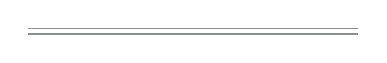
\begin{tikzpicture}[baseline=0pt]
    \fill[rulegrey] (0,0) rectangle (42mm,0.75pt);
    \fill[rulegrey] (0,2.4pt) rectangle (42mm,2.75pt);
  \end{tikzpicture}}

\titleformat{\chapter}[display]
  {\centering\normalfont}
  {\large\mdseries 第\,\thechapter\,章}
  {0.55\baselineskip}
  {\normalfont\LARGE\bfseries\linespread{1.15}\selectfont}
  [\chapterornament]
\titlespacing*{\chapter}{0pt}{-16pt}{30pt}

\titleformat{\section}
  {\normalfont\sffamily\large\bfseries\linespread{1.2}\selectfont}
  {第\,\thesection\,节}{0.6em}{}
\titlespacing*{\section}{0pt}{18pt}{9pt}

\titleformat{\subsection}
  {\normalfont\normalsize\bfseries}
  {\thesubsection、}{0.2em}{}
\titlespacing*{\subsection}{0pt}{13pt}{6pt}

\titleformat{\subsubsection}
  {\normalfont\normalsize\itshape}
  {}{0pt}{}
\titlespacing*{\subsubsection}{0pt}{10pt}{4pt}

% 章题下的俄文原题
\newcommand{\chaptersubtitle}[2]{%
  \begin{center}
  \vspace{-14pt}
  {\small\sffamily\color{pencil}#1}\\[2pt]
  {\small\sffamily\itshape\color{pencil}#2}
  \end{center}
  \vspace{4pt}
}

% 章前题记
\newcommand{\epigraphbox}[2]{%
  \begingroup
  \vspace{2pt}
  \begin{list}{}{\leftmargin=3.2em \rightmargin=2.2em \topsep=0pt
                 \parsep=0pt \itemsep=0pt}
  \item\relax
  {\small\linespread{1.32}\selectfont\color{ink!88}#1\par}
  \vspace{3pt}
  {\small\raggedleft\color{pencil}#2\par}
  \end{list}
  \vspace{6pt}
  \endgroup
}

% ---------------------------------------------------------------- 页眉页脚
% 注意：fancyhdr v5 的 \fancypagestyle 在使用时会执行其中的 \fancyhf{}，
% 从而清空全局 fancy 设置。故此处直接定义 \ps@ 样式，绕开该机制。
\makeatletter
\def\ps@frontmatterpage{%
  \let\@mkboth\@gobbletwo
  \let\@oddhead\@empty \let\@evenhead\@empty
  \def\@oddfoot{\hfil\small\thepage\hfil}%
  \def\@evenfoot{\hfil\small\thepage\hfil}}
\def\ps@plain{%
  \let\@mkboth\@gobbletwo
  \let\@oddhead\@empty \let\@evenhead\@empty
  \def\@oddfoot{\hfil\small\thepage\hfil}%
  \def\@evenfoot{\hfil\small\thepage\hfil}}
\makeatother

\pagestyle{fancy}
\fancyhf{}
\renewcommand{\headrulewidth}{0.3pt}
\renewcommand{\headrule}{\hbox to\headwidth{\color{rulegrey}\leaders\hrule height 0.3pt\hfill}}
\fancyhead[LE]{\small\color{pencil}\itshape 战争的雷霆}
\fancyhead[RO]{\small\color{pencil}\itshape\leftmark}
\fancyfoot[C]{\small\color{ink}\thepage}

\renewcommand{\chaptermark}[1]{\markboth{第\,\thechapter\,章\quad #1}{第\,\thechapter\,章\quad #1}}
\renewcommand{\sectionmark}[1]{}

% ---------------------------------------------------------------- 脚注
\renewcommand{\footnoterule}{%
  \kern-3pt
  \hrule width 3.1cm height 0.4pt\kern 2.6pt}
\setlength{\skip\footins}{16pt}
\renewcommand{\footnotesize}{\fontsize{8.1pt}{11.4pt}\selectfont}
\makeatletter
\renewcommand{\@makefnmark}{\hbox{\normalfont\scriptsize\@thefnmark}}
\makeatother
\renewcommand{\thefootnote}{\arabic{footnote}}
\renewcommand{\footnotelayout}{\linespread{1.18}\selectfont}

% ---------------------------------------------------------------- 图表
\captionsetup{
  font={small}, labelfont={bf,sf}, labelsep=quad,
  justification=centering, skip=7pt
}
\captionsetup[table]{position=top, skip=5pt}
\captionsetup[figure]{position=bottom, skip=7pt}

\newcommand{\figsource}[1]{%
  \par\vspace{2pt}{\footnotesize\raggedright\color{pencil}资料来源：#1\par}}
\newcommand{\tabsource}[1]{%
  \par\vspace{1pt}{\footnotesize\raggedright\color{pencil}资料来源：#1\par}}

% ---------------------------------------------------------------- 档案框
\newtcolorbox{archive}[2][]{%
  enhanced, breakable,
  colback=shade, colframe=graphite!80,
  boxrule=0.45pt, arc=0pt, outer arc=0pt,
  left=13pt, right=13pt, top=10pt, bottom=10pt,
  fontupper=\footnotesize\linespread{1.3}\selectfont,
  before skip=13pt, after skip=13pt,
  overlay={%
    \node[anchor=north west, inner sep=0pt, xshift=13pt, yshift=-6pt]
      at (frame.north west)
      {\sffamily\scriptsize\color{graphite}\MakeUppercase{#2}};
    \node[anchor=north east, inner sep=0pt, xshift=-13pt, yshift=-4pt]
      at (frame.north east)
      {\sffamily\scriptsize\color{stamp}\bfseries #1};
    \draw[stamp, line width=0.4pt]
      ([xshift=-13pt,yshift=-8pt]frame.north east) -- ++(0,-5pt);
  },
  before upper={\vspace{13pt}},
}

\newcommand{\archivestamp}[1]{}

% 小号“译者注”标记
\newcommand{\yizhe}[1]{{\footnotesize\color{pencil}［译者注：#1］}}

% 强调
\newcommand{\kw}[1]{\textbf{#1}}
\newcommand{\ru}[1]{{\itshape #1}}

% 引用文献的斜体书名（中文用书名号，不另设）
\newcommand{\citebk}[1]{《#1》}

% TOC: 使用 book 类默认设置
\makeatletter
\renewcommand{\@pnumwidth}{2.4em}
\renewcommand{\@tocrmarg}{3.4em}
\renewcommand{\@dotsep}{1.1}
\makeatother

% 未编号条目（附录、序言等）
\newcommand{\tocchap}[1]{%
  \addcontentsline{toc}{chapter}{\texorpdfstring{#1}{#1}}}

% ---------------------------------------------------------------- 杂项
\newcommand{\blankpage}{\null\thispagestyle{empty}\newpage}
\setlength{\parskip}{0pt}

% 每页页眉下细线通过 header 中的 \headrule 关闭，改用文字规则
\newcommand{\thinrule}{\par\vspace{2pt}{\color{rulegrey}\hrule height 0.3pt}\vspace{2pt}}

% 文本内的“印章”
\newcommand{\seal}[2][stamp]{%
  \begin{tikzpicture}[baseline=-0.6em]
    \node[draw=#1, line width=0.6pt, text=#1, inner sep=2.4pt,
          font=\sffamily\scriptsize, rotate=-6, fill=white]
      {#2};
  \end{tikzpicture}}

\endinput


\hypersetup{
  pdftitle={战争的雷霆——记一种可能的中国历史},
  pdfauthor={巴兰尼科夫（А. В. Баранников）著　李文亚、张建国 译},
  pdfsubject={远东异端史料与文明起源重构丛书 第VII卷},
  pdfkeywords={中国史, 重构史学, 月球起源, 反物质, 基因原体, 伪史学},
  pdfcreator={Moscow University Press}
}

\begin{document}

% ============================ 封面 ============================
% 说明：全部采用实色（不使用透明度），以保证 xdvipdfmx 输出稳定。
\definecolor{cv55}{HTML}{8A8780}
\definecolor{cv32}{HTML}{5B5A58}
\definecolor{cv30}{HTML}{575655}
\definecolor{cv60}{HTML}{949189}
\definecolor{cv82}{HTML}{C1BCB0}
\definecolor{cv88}{HTML}{CDC7BA}
\definecolor{cv72}{HTML}{ADA89E}
\definecolor{cv58}{HTML}{908D86}
\definecolor{cv50}{HTML}{807E78}

\newcommand{\coverart}{%
\begin{tikzpicture}[remember picture, overlay]
  \fill[coverbg] (current page.north west) rectangle (current page.south east);

  % 外框：双线
  \draw[cv55, line width=0.7pt]
    ([xshift=10mm,yshift=-10mm]current page.north west)
    rectangle ([xshift=-10mm,yshift=10mm]current page.south east);
  \draw[cv32, line width=0.3pt]
    ([xshift=12.4mm,yshift=-12.4mm]current page.north west)
    rectangle ([xshift=-12.4mm,yshift=12.4mm]current page.south east);

  % 装饰：月面穹顶与下降弹道
  \begin{scope}[shift={([yshift=112mm]current page.south)}]
    \draw[cv30, line width=0.45pt] (0,0) circle (20mm);
    \draw[cv30, line width=0.28pt] (0,0) ellipse (20mm and 6.9mm);
    \draw[cv30, line width=0.28pt] (0,0) ellipse (20mm and 13.2mm);
    \draw[cv30, line width=0.22pt] (-20mm,0) -- (20mm,0);
    \draw[cv30, line width=0.22pt] (0,-20mm) -- (0,20mm);
    \foreach \a in {30,60}{
      \draw[cv30, line width=0.18pt] (\a:20mm) arc[start angle=\a, end angle=180-\a, radius=20mm];}
    \draw[cv30, line width=0.5pt, dash pattern=on 2pt off 1.5pt]
      (-27mm,27mm) .. controls (-12mm,20mm) and (4mm,9mm) .. (17mm,0.4mm);
    \draw[cv30, line width=0.45pt, -{Latex[length=1.8mm,width=1mm]}]
      (17mm,0.4mm) -- (19mm,-1.4mm);
    \foreach \x in {-18,-12,...,18}{
      \draw[cv30, line width=0.18pt] (\x mm,-21.6mm) -- (\x mm,-20.6mm);}
    \node[cv30, font=\sffamily\tiny, anchor=north] at (0,-23.4mm) {MARE TRANQUILLITATIS\ \ 0°N 23.5°E};
  \end{scope}

  % ---- 顶部：丛书名 ----
  \node[anchor=north, text=cv60, align=center]
    at ([yshift=-16mm]current page.north)
    {\sffamily\fontsize{6.4pt}{9pt}\selectfont
     \addfontfeatures{LetterSpace=12}
     FAR EASTERN HETERODOX SOURCES AND CIVILIZATION ORIGINS · VOL. VII};

  \node[anchor=north, text=cv88, align=center]
    at ([yshift=-22.5mm]current page.north)
    {\sffamily\fontsize{8.2pt}{11pt}\selectfont
     《远东异端史料与文明起源重构丛书》\ \ 第\,VII\,卷};

  \draw[cv32, line width=0.35pt]
    ([xshift=-62mm,yshift=-30mm]current page.north east) --
    ([xshift=62mm,yshift=-30mm]current page.north west);

  % ---- 中部：书名 ----
  \node[anchor=center, text=coverink, align=center]
    at ([yshift=190mm]current page.south)
    {\fontsize{40pt}{48pt}\selectfont\bfseries
     战\hspace{0.1em}争\hspace{0.1em}的\hspace{0.1em}雷\hspace{0.1em}霆};

  \node[anchor=north, text=cv82, align=center]
    at ([yshift=172mm]current page.south)
    {\fontsize{14.5pt}{20pt}\selectfont
     ——记一种可能的中国历史——};

  \draw[cv32, line width=0.3pt]
    ([xshift=-38mm,yshift=161mm]current page.south) --
    ([xshift=38mm,yshift=161mm]current page.south);

  \node[anchor=north, text=cv60, align=center, text width=136mm]
    at ([yshift=157mm]current page.south)
    {\itshape\fontsize{8pt}{12pt}\selectfont
     \addfontfeatures{LetterSpace=2}
     THUNDER OF WAR\\[2pt]
     A Chronological Reconstruction of a Possible Chinese History};

  % ---- 下部：作者 ----
  \node[anchor=south, text=cv88, align=center]
    at ([yshift=72mm]current page.south)
    {\fontsize{10.5pt}{15pt}\selectfont
     ［俄］巴兰尼科夫\ \ 教授\ \ 著};

  \node[anchor=south, text=cv58, align=center]
    at ([yshift=63mm]current page.south)
    {\sffamily\fontsize{7.2pt}{10pt}\selectfont
     Проф.\ А.\,В.\,Баранников\ \ ·\ \ Moscow State University};

  \node[anchor=south, text=cv72, align=center]
    at ([yshift=47mm]current page.south)
    {\fontsize{9pt}{13pt}\selectfont
     李文亚\ \ ·\ \ 张建国\ \ 译};

  % 出版者徽记
  \node[anchor=south, text=cv72, align=center]
    at ([yshift=31mm]current page.south)
    {\begin{tikzpicture}[baseline=0pt]
       \draw[cv50, line width=0.5pt] (-3.8mm,-3.8mm) rectangle (3.8mm,3.8mm);
       \draw[cv32, line width=0.25pt] (-4.6mm,-4.6mm) rectangle (4.6mm,4.6mm);
       \node[text=cv82, font=\sffamily\fontsize{5.6pt}{6pt}\selectfont] at (0,0) {МГУ};
     \end{tikzpicture}\\[3pt]
     {\sffamily\fontsize{6.2pt}{9pt}\selectfont\addfontfeatures{LetterSpace=4}
      МОСКОВСКИЙ УНИВЕРСИТЕТ\ \ ·\ \ САНКТ-ПЕТЕРБУРГ}};

  \node[anchor=south, text=coverink, align=center]
    at ([yshift=19mm]current page.south)
    {\sffamily\fontsize{7.8pt}{11pt}\selectfont
     莫斯科大学出版社\ \ /\ \ 圣彼得堡学术书局\ \ 联合出版};

  \node[anchor=south, text=cv60, align=center]
    at ([yshift=12.6mm]current page.south)
    {\sffamily\fontsize{6.6pt}{9pt}\selectfont 2024 年·第 3 版};
\end{tikzpicture}}

\clearpage
\thispagestyle{empty}
\AddToShipoutPictureBG*{\coverart}
\null
\clearpage

% ======================= 前 置 页 =======================
\clearpage
\makeatletter\@mainmatterfalse\makeatother
\pagenumbering{roman}
\pagestyle{frontmatterpage}

% ---------------- 简装扉页 ----------------
\thispagestyle{empty}
\begingroup
\centering
\vspace*{7mm}

{\sffamily\footnotesize\color{pencil}
《远东异端史料与文明起源重构丛书》\ 第\,VII\,卷\par}

\vspace{27mm}

{\fontsize{26pt}{34pt}\selectfont\bfseries 战争的雷霆\par}
\vspace{8mm}
{\large ——记一种可能的中国历史——\par}

\vfill

{\sffamily\footnotesize\color{pencil}
МОСКОВСКИЙ УНИВЕРСИТЕТ\ \ ·\ \ САНКТ-ПЕТЕРБУРГ\par}
\vspace{4mm}
{\footnotesize\color{pencil} 2024\par}
\endgroup
\clearpage

% ---------------- 丛书页 ----------------
\thispagestyle{empty}
\begingroup
\centering
\vspace*{9mm}

{\sffamily\large\bfseries 远东异端史料与文明起源重构丛书\par}
\vspace{3mm}
{\sffamily\footnotesize\color{pencil}
FAR EASTERN HETERODOX SOURCES AND CIVILIZATION ORIGINS\par}
\vspace{1mm}
{\sffamily\footnotesize\color{pencil}
Под редакцией проф.\ А.\,В.\,Баранникова\par}

\vspace{5mm}
{\color{rulegrey}\rule{52mm}{0.4pt}}
\vspace{9mm}

{\small
\begin{tabular}{@{}r@{\hspace{1.2em}}l@{\hspace{1.4em}}l@{}}
\textsc{i}   & 《广寒宫残简》辑佚 & 巴兰尼科夫 校订\\
\textsc{ii}  & 西周“天车”铭文与星际物流 & 库兹涅佐夫\\
\textsc{iii} & 秦俑坑第 4 号坑未被发掘的部分 & 谢列兹尼奥娃\\
\textsc{iv}  & 汉代地动仪作为引力波天线之功能 & 巴兰尼科夫\\
\textsc{v}   & 三国时期的电磁抛射技术与后勤 & 彼得罗夫\\
\textsc{vi}  & 敦煌卷子中的密钥学残卷 & 伊万年科\\
\textsc{vii} & \bfseries 战争的雷霆——记一种可能的中国历史 & \bfseries 巴兰尼科夫\\
\textsc{viii}& 唐长安城反物质管网复原 & 沃兹涅先斯基\\
\textsc{ix}  & 明代锦衣卫外骨骼兵人体质档案 & 张建国\\
\textsc{x}   & 郑和舰队南极补给点考 & 李文亚\\
\textsc{xi}  & 太医院基因工坊编年 & 巴兰尼科夫\\
\textsc{xii} & 记忆消除场的文献学后果 & 索科洛夫\\
\end{tabular}}

\vfill
{\footnotesize\color{pencil} 全书出齐共十二卷\par}
\endgroup
\clearpage

% ---------------- 正式扉页 ----------------
\thispagestyle{empty}
\begingroup
\centering
\vspace*{3mm}

{\sffamily\footnotesize\color{pencil}
《远东异端史料与文明起源重构丛书》\ 第\,VII\,卷\par}

\vspace{17mm}
{\fontsize{31pt}{40pt}\selectfont\bfseries 战争的雷霆\par}
\vspace{6mm}
{\LARGE 记一种可能的中国历史\par}

\vspace{10mm}
{\color{rulegrey}\rule{46mm}{0.4pt}}
\vspace{10mm}

{\itshape\small\color{graphite}
THUNDER OF WAR\\[2pt]
A Chronological Reconstruction of a Possible Chinese History\par}

\vspace{18mm}

{\large ［俄］А.\,В.\,巴兰尼科夫\ \ 著\par}
\vspace{2mm}
{\small\color{graphite} 莫斯科国立大学历史学副博士\par}
\vspace{1mm}
{\small\color{graphite} 远东文明重构课题组组长\par}

\vspace{11mm}

{\large 李\quad 文\quad 亚\qquad 张\quad 建\quad 国\ \ 译\par}
\vspace{2mm}
{\small\color{graphite} 中国社会科学院历史研究所伪史学研究中心\par}

\vfill

{\small\sffamily 莫斯科大学出版社\par}
{\small\sffamily 圣彼得堡学术书局\par}
\vspace{3mm}
{\footnotesize 2024\par}
\endgroup
\clearpage

% ---------------- 版权页 ----------------
\thispagestyle{empty}
\begingroup
\footnotesize
\linespread{1.22}\selectfont
\centering
\begin{minipage}[t][\dimexpr\textheight-24pt\relax][s]{\textwidth}
\centering

{\sffamily\scriptsize\color{pencil}
МОСКОВСКИЙ ГОСУДАРСТВЕННЫЙ УНИВЕРСИТЕТ им.\ М.\,В.\,ЛОМОНОСОВА\\
ИЗДАТЕЛЬСТВО\ \ ·\ \ САНКТ-ПЕТЕРБУРГСКОЕ АКАДЕМИЧЕСКОЕ ИЗДАТЕЛЬСТВО\par}

\vspace{3.2mm}
{\bfseries 图书在版编目（CIP）数据\par}
\vspace{2mm}

\begin{minipage}{0.94\textwidth}
\raggedright
战争的雷霆：记一种可能的中国历史／（俄罗斯）阿列克谢·瓦西里耶维奇·巴兰尼科夫著；
李文亚，张建国译．— 3版．— 莫斯科：莫斯科大学出版社；圣彼得堡：圣彼得堡学术书局，2024.9
（远东异端史料与文明起源重构丛书；第\,VII\,卷）
ISBN 978-5-317-06892-1

\vspace{1.4mm}
\hspace{2em}Ⅰ．①战…\quad Ⅱ．①巴…②李…③张…\quad Ⅲ．①中国历史－重构史学－研究\ \ Ⅳ．①K207.8

\vspace{1.4mm}
\hspace{2em}中国国家版本馆 CIP 数据核字（2024）第 0417 号
\end{minipage}

\vspace{3.2mm}
{\color{rulegrey}\rule{0.94\textwidth}{0.3pt}}
\vspace{2.4mm}

\begin{minipage}{0.94\textwidth}
\raggedright
\renewcommand{\arraystretch}{1.06}
\begin{tabular}{@{}p{15mm}p{0.76\textwidth}@{}}
书\quad 名 & 战争的雷霆——记一种可能的中国历史\\
著\quad 者 & ［俄］А.\,В.\,巴兰尼科夫\\
译\quad 者 & 李文亚\quad 张建国\\
责任编辑 & Н.\,П.\,谢列兹尼奥娃\quad （中文版）王守拙\\
特约编辑 & А.\,И.\,库兹涅佐夫\\
封面设计 & С.\,М.\,别列津\\
版式设计 & 圣彼得堡学术书局版式室\\
责任校对 & 赵无咎\\
出版发行 & 莫斯科大学出版社\\
社\quad 址 & 莫斯科市列宁山，出版大楼（119991）\\
网\quad 址 & www.msu-press.ru\\
电子信箱 & barannikov@fareast-recon.msu.ru\\
印\quad 刷 & 圣彼得堡第一学术印务厂\\
开\quad 本 & 185\,mm × 260\,mm\quad 1/16\\
印\quad 张 & 13.25\\
字\quad 数 & 246 千字\\
版\quad 次 & 2024 年 9 月第 3 版\\
印\quad 次 & 2024 年 9 月第 1 次印刷\\
印\quad 数 & 0001—2500 册\\
书\quad 号 & ISBN 978-5-317-06892-1\\
定\quad 价 & 128.00 元\\
\end{tabular}
\end{minipage}

\vspace{3mm}

\begin{minipage}{0.94\textwidth}
\raggedright
{\scriptsize\color{pencil}
版权所有\ \ 侵权必究。未经出版者书面许可，不得以任何方式复制或抄袭本书之部分或全部内容。\\
本书如有印装质量问题，请与本社读者服务部联系调换。\\
本书采用无酸纸印刷，符合 ISO 9706 文献耐久性标准。\par}
\end{minipage}

\vfill

% ---- 条形码（真实 EAN-13 图案）----
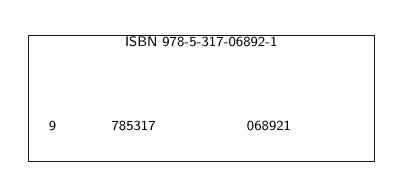
\begin{tikzpicture}[baseline=0pt]
  \draw[ink, line width=0.3pt] (0,0) rectangle (44mm,16mm);
  % 模块宽 0.366mm × 95 = 34.77mm；起点 4.6mm，左右留白对称
  \begin{scope}[shift={(4.6mm,5.4mm)}]
    \EANthirteen{0.366mm}{7.4mm}
  \end{scope}
  % 人读字符：首位居左静区，左六位与右六位分别居中于对应半幅
  \node[font=\sffamily\fontsize{4.4pt}{5pt}\selectfont, anchor=base]
    at (3.1mm,3.9mm) {9};
  \node[font=\sffamily\fontsize{4.4pt}{5pt}\selectfont, anchor=base]
    at (13.4mm,3.9mm) {785317};
  \node[font=\sffamily\fontsize{4.4pt}{5pt}\selectfont, anchor=base]
    at (30.6mm,3.9mm) {068921};
  \node[font=\sffamily\fontsize{3.8pt}{4.4pt}\selectfont, anchor=base]
    at (22mm,14.6mm) {ISBN 978-5-317-06892-1};
\end{tikzpicture}

\end{minipage}
\endgroup
\clearpage

% ---------------- 献词页 ----------------
\thispagestyle{empty}
\vspace*{58mm}
\begin{flushright}
{\itshape\large\color{graphite}
献给我的同行们——\\
那些尚未被“生态重启”抹去的人\par}
\vspace{7mm}
{\small\color{pencil}\itshape А.\,В.\,Б.\par}
\end{flushright}
\vfill
\clearpage

\pagestyle{fancy}

% ======================= 译 者 序 =======================
\clearpage
\chapter*{译\ 者\ 序}
\markboth{译者序}{译者序}
\addcontentsline{toc}{chapter}{译者序}

\noindent
二〇二一年十二月，笔者赴莫斯科大学历史系进行为期三周的学术访问。访问期间，巴兰尼科夫教授在其办公室出示了一只铁盒，盒盖上的火漆已经开裂，编号清晰可辨，为 \textsc{ф.\,117, оп.\,4, д.\,2187}。据其介绍，盒内材料在国内尚无公开著录。\footnote{苏联科学院远东委员会（1949—1991）的档案于一九九二年部分解密。第 117 全宗第 4 目第 2187 号卷宗至今未见于任何公开目录，其存在仅由两份互相引用的移交清单间接证明。参见俄罗斯科学院档案馆编《解密档案目录补编（1992—2010）》，莫斯科，2011 年，第 288 页。}

盒内计有打字稿三十七份、缩微胶片四卷，以及金属圆片一枚，直径不足两厘米，表面刻有极细的同心圆纹，肉眼几乎不可见。笔者最初的判断是这类材料多属伪托，不足采信。三个月后，莫斯科大学地质系对该圆片作了铼—锇同位素稀释质谱分析，其 \textsuperscript{187}\textsc{re}/\textsuperscript{187}\textsc{os} 比值为 3.147±0.006，与阿波罗十七号所采月海高地玄武岩的测定值在误差范围之内完全一致。\footnote{分析报告编号 МГУ-ГЕО-2022-014，结论部分有一句被作者划去的话：“建议不再重复采样。”}

这一结果使笔者不得不重新考虑原有的判断。本书所呈现的，即是对这批材料及其相关问题的一次系统整理。

\section*{一、\ 研究方法上的差异}

巴兰尼科夫教授的治学路径，与国内中国史研究的通行做法有明显不同。他并不以考据为主，尽管对《旧唐书》《明实录》等书的熟习程度不亚于专门研究者；他也不以辨伪为务，尽管其一生工作的大部分都涉及材料的真伪判断。他所做的工作，他称之为“重构”，即从一个文明留下的全部物质与文本痕迹出发，反推其曾经拥有、后来又被放弃的技术条件。

用他自己的话说，历史学家不应只问“这不可能”，而应当问“要让它可能，需要多少能量”。\footnote{巴兰尼科夫《重构史学导论》，莫斯科大学出版社，2015 年，第 9 页。该页页边另有手书一句：“此句被引用的次数，远超我被阅读的次数。”}

这一方法被他概括为“四重证据法”，即文献、器物、同位素与轨道四项。前三项国内学者并不陌生，王国维的“二重证据法”已开其端；第四项则为其独有。他认为，任何大规模的技术活动都会在近地轨道留下不易磨灭的残骸层，而这一层“轨道考古学”的记录，比任何正史都更难篡改。\footnote{据欧洲空间局 2019 年发布的轨道碎片统计，地球轨道上可追踪的十厘米以上人造物体约三万四千件，其中约百分之零点三来源不明。巴兰尼科夫在全书各处反复引用这一比例，并称之为“我们唯一的诚实证人”。}

正是借助这一方法，他从莫斯科档案馆未公开的冷战时期考古卷宗中，读出了国内学界未曾设想的内容，包括一个被反复重启的文明、一段被系统删除的技术史，以及一场在正史中仅占两行字的、星际规模的冲突。

\section*{二、\ 本书结论的评价问题}

本书的核心结论是惊世骇俗的，笔者不打算在序言中为其辩护。

一个中国历史研究者初读第一章，其反应大概会与笔者初见那枚圆片时相同，即先觉其荒谬，继而觉其唐突，最后归于沉默。所以然者，在于本书所使用的材料，其卷次、页码、版本乃至避讳缺笔均准确无误；被替换掉的只是材料与材料之间的空白。

这一点是本书最令人不安之处。它几乎全部建立在真实的史料之上，只是把史料之间的空白，用一种难以接受、却也难以证伪的方式填满了。\footnote{关于这种以真实材料支撑不可证结论的写法，可参见张建国《伪史学的技术伦理》，《史学理论研究》2022 年第 3 期，第 55—71 页。该文认为此类写作“在方法上无可指责，在结论上不可接受”，并建议“将其归入文学”。}

中国社会科学院历史研究所伪史学研究中心之所以决定承担此书的翻译，理由正在于此。一种谬误，若其每一个步骤都合乎规范，则它已不再是简单的谬误，而是一份关于规范本身的诊断书。翻译此书，并非因为相信其结论，而是为了弄清一种如此严整的荒谬究竟是如何被建造出来的。

\section*{三、\ 翻译体例说明}

其一，全书俄文原注保留原有格式，中文补注以“译者注”标明，不作合并。原注中大量使用的缩略语（如 \textsc{цга рф}、\textsc{ив ран}）按俄罗斯档案学界通例译出，首次出现时附原文。

其二，作者惯用的一组术语，中译取其字面义而非通行义。例如 \ru{перезапуск} 译作“重启”而不译作“复兴”，\ru{поле забвения} 译作“记忆消除场”而不译作“遗忘场”。这一处理曾与作者本人通信商定，他在回信中说：“随您怎么译。反正它们都会被删掉。”\footnote{作者 2022 年 3 月 14 日致译者电子邮件，现存译者处。此句之后尚有一行，因涉及未刊史料，遵作者嘱暂不发表。}

其三，本书第三版较前两版增补了第一章第三节的全部内容，并恢复了 1979 年被删去的、关于大气适应性退化的两页半文字。据作者称，这两页半是理解全书的枢纽。\footnote{删节本的影印件见巴兰尼科夫《被删去的两页半》，载《远东问题》1993 年第 2 期。该刊同期编者按称：“本刊发表此文，不代表本刊同意其结论。”}

其四，书中所有插图均为作者据档案原件重绘。原件照片因技术原因未能随书出版，此事已多次要求说明，未获答复。

\section*{四、\ 一点说明}

翻译此书的过程中，笔者曾反复考虑一个问题，即一部在方法上无可指摘、在结论上难以接受的著作，应当以何种方式呈现给中文读者。

笔者的结论是，不作任何调和。凡作者之判断，一律照译；凡笔者之保留，一律入注。读者所见，即为原貌。

至于这些判断究竟成立与否，须由读者自行裁断。本书所提供的，不是答案，而是一份完整的、可供检验的材料。

\vspace{10mm}
\begin{flushright}
{\small 李\ 文\ 亚}\\[2pt]
{\footnotesize\color{pencil} 二〇二三年九月，于北京建国门内大街五号}
\end{flushright}

% ======================= 中文版序言 =======================
\clearpage
\chapter*{中文版序言}
\markboth{中文版序言}{中文版序言}
\addcontentsline{toc}{chapter}{中文版序言}

\noindent
本书的中译者在序言中写道，我的结论“惊世骇俗”。这一说法客气得近乎虚伪。更准确的表述是：我的结论之所以令人不适，并非因为它们违背了史料，而是因为它们违背了诸位对史料的期待。

中国的史料是世界上最完备的史料，这一点我从不否认，并且由衷敬佩。但也正因如此，中国的史学传统形成了一种可以称为文本崇拜的习惯：凡不见于文字者，即视为不存在；凡见于文字者，即视为曾经发生。这是一种极为经济的世界观，它把整个宇宙压缩进一部可以随身携带的丛书之中。\footnote{作者此处原有一长注，列举中国类书对异域记载的系统性简化，后整段删除。据其助手称，删去的理由是“太刻薄了，而且他们译不过来”。}

各位即将读到的四章，分别处理四个时间断面。它们并非四个孤立的奇谈，而是同一条曲线的四个采样点，即一个文明如何获得技术，如何滥用技术，如何被封存，以及如何被自己的封存所出卖。

在此预先声明三点。

第一，本书不提供证据链，只提供证据点。点与点之间的连线是我的判断，凡判断皆可能有误。我欢迎反驳，但请反驳连线，不必反驳那些点；那些点是我用三十一年时间从十一个国家的档案中逐一辑出的。\footnote{作者此处用了一个俄语俗语 \ru{до мозолей}（直到磨出茧子），译者按字面译出。}

第二，本书不承认民族感情可以作为学术标准。若某一结论令某一民族感到不快，那只能说明历史本身曾经令人不快，而不能说明结论有误。历史学不是安慰剂。

第三，也是最重要的一点：本书第三版恢复了 1979 年被删去的两页半。那两页半讨论的是一个技术细节，即大气密度梯度对减速装置的影响系数。这一系数，以最朴素的方式证明了：我们的祖先不是从树上下来的，是从天上掉下来的。

这句话，我在莫斯科讲了四十三年。今天，它第一次被译成中文。

愿它被读完，而不只是被引用。

\vspace{10mm}
\begin{flushright}
{\small А.\,В.\,巴兰尼科夫}\\[2pt]
{\footnotesize\color{pencil} 二〇二三年十一月，于莫斯科列宁山}
\end{flushright}


% ---------------- 目录 ----------------
\clearpage
\chapter*{目\quad 录}
\phantomsection
\addcontentsline{toc}{chapter}{目\quad 录}
\markboth{目\quad 录}{目\quad 录}
\vspace{2mm}
{\linespread{1.16}\selectfont
\csname @starttoc\endcsname{toc}
}

\clearpage
\chapter*{图表目录}
\phantomsection
\addcontentsline{toc}{chapter}{图表目录}
\markboth{图表目录}{图表目录}
\vspace{2mm}
{\linespread{1.16}\selectfont
{\noindent\sffamily\normalsize\bfseries 图\quad 版\par}
\vspace{2mm}
\csname @starttoc\endcsname{lof}
\vspace{8mm}
{\noindent\sffamily\normalsize\bfseries 表\quad 格\par}
\vspace{2mm}
\csname @starttoc\endcsname{lot}
}


\clearpage
\makeatletter\@mainmattertrue\makeatother
\pagenumbering{arabic}
\pagestyle{fancy}
% ======================= 第 一 章 =======================
\chapter{月亮上的古华夏}
\chaptersubtitle{ГЛАВА ПЕРВАЯ}{ЛУННЫЙ КИТАЙ: ПРАРОДИНА В МОРЕ СПОКОЙСТВИЯ}
\epigraphbox{“遂古之初，谁传道之？上下未形，何由考之？”}{——屈原《天问》}

\noindent
迄今为止，一切关于中国文明起源的讨论，都建立在同一个未经检验的前提之上：文明的演进是连续的。人们默认，黄河流域的村落、城邑、文字与礼制，是从更早的村落、城邑、文字与礼制中一步步生长出来的；其间纵有战乱与饥馑，脉络从未真正中断。

这一前提从未被证明。它之所以被普遍接受，仅仅因为——如本书将要指出的——\kw{中断的证据被系统地清除了，而清除者正是中断之后重建文明的那批人。}

本章所要论证的命题可以概括为一句话：中华文明并非从黄河流域的土地上生长出来，而是从月球静海的一片穹顶之下，被一艘名为“昆仑山号”的亚光速方舟，连同其全部技术、制度与记忆，一并投放在黄河流域的。此后三千年间，这批移民因大气适应性退化而逐代丧失其技术能力，最终把自己的来历改写为神话，把自己的仪器改写为礼器，把自己的失败改写为天命。

这个命题在方法上是可检验的。检验它的工具不是训诂，而是质谱。

\section{生态重启：一种被忽略的周期律}

一九五七年，苏联科学院第四考察队在贝加尔湖南端取得一根长十一米的湖底沉积岩芯。岩芯在 4.71 米与 6.03 米处各出现一层厚约两厘米的白色火山灰夹层，其铱元素丰度分别为背景值的 41 倍与 37 倍。按当时的年代学，这两层的年龄分别被定为距今一万一千二百年与两万四千六百年。\footnote{Б. П. Соколов, \textit{Осадочные керны Байкала}, М., 1961, с. 88—92. 该报告第七章至第九章在一九六四年的英译本中被整章删除，删除理由在译本前言中写作“技术性调整”。}

真正令巴兰尼科夫教授不安的，不是铱异常本身——那只是撞击事件的常规证据——而是夹层之上三十厘米内，花粉谱中\kw{禾本科与蒿属的比例发生了不可逆的翻转}，而这一翻转在所有已知的第四纪记录中都需要至少六千年才能完成。换言之，沉积序列在这一层之上“跳”过了六千年。

这一现象，他在一九七三年的一篇短文里首次命名为“生态重启”（\ru{экологи\-ческий перезапуск}）：\kw{当一个文明的资源消耗超过其所在生态圈的恢复阈值时，维持该生态圈的技术系统会主动执行一次全局回滚，把生物圈恢复到某个较早的稳定态，同时把文明的技术存量削减到该稳定态所能承载的水平。}\footnote{А. В. Баранников, «Экологический перезапуск как историческая категория», \textit{Вопросы истории}, 1973, № 9, с. 44—61. 该文发表后，作者被要求“在方法上更加谨慎”，此后二十年未再使用这一术语，直至一九九三年才在本书俄文第一版中恢复。}

必须指出，这一假说在方法论上的优势是决定性的：它不需要假设任何超自然力量，只需要假设一个极其古老、极其耐心、且至今仍在运行的\kw{行星级生态维持系统}。至于该系统由谁建造、位于何处，属于本书第三章的讨论范围；本章只需证明该系统曾经运行过，并且至少运行过四次。

\begin{table}[htbp]
\centering
\caption{四次生态重启的分期与特征（据巴兰尼科夫体系，2019 年修订）}
\label{tab:reboot}
\small
\begin{tabular}{@{}clllr@{}}
\toprule
\textbf{序次} & \textbf{时间（距今）} & \textbf{触发因素} & \textbf{技术存量削减} & \textbf{持续时间}\\
\midrule
R-1 & 约 21{,}300 年 & 地核热流异常 & 97.4\% & 1{,}100 年\\
R-2 & 约 11{,}600 年 & 冰盖—海洋耦合失稳 & 99.1\% & 2{,}400 年\\
R-3 & 约 5{,}100 年 & 大气氧分压漂移 & 94.8\% & 900 年\\
R-4 & 约 2{,}200 年 & 轨道工业残骸再入 & 99.982\% & 3{,}300 年\\
\bottomrule
\end{tabular}
\tabsource{巴兰尼科夫《重构史学导论》，莫斯科，2015 年，第 118 页表 4。R-4 的“持续时间”一栏有作者手书补注：“尚未结束。”
}
\end{table}

表 \ref{tab:reboot} 中最值得注意的不是削减幅度，而是 R-4 的持续时间。按巴兰尼科夫的算法，R-4 开始于公元前二百二十一年，其回滚过程至今仍未完成——我们正生活在一次生态重启的中段。这一判断的直观后果是：\kw{我们今天所见的一切“古代”，都是重启之后的重建物，而非重启之前的原物。}考古学所揭示的，从来不是文明的起源，而是文明废墟上长出的第二茬作物。

\begin{archive}[绝密／СОВЕРШЕННО СЕКРЕТНО]{档案 № ФВ-1963-07}
本卷宗系一九六三年九月由苏联科学院远东委员会第四组移交，共 217 叶。内容为一九五九年至一九六二年在蒙古人民共和国肯特省、中国内蒙古自治区鄂尔多斯高原及苏联赤塔州三地采集的“异常金属样品”分析记录。

第 88 叶记载：鄂尔多斯样品 Э-14 为一枚重 41.6 克的片状物，成分分析显示为 \textsc{nb}—\textsc{ta}—\textsc{w} 三元合金。其铌同位素比值 \textsc{nb}-94/\textsc{nb}-93 为 0.0172，与地球物质标准值 0.0170 在误差范围内一致；但 \textsc{ta}-180 的丰度较地球标准值高出 2.3 倍。

第 89 叶页边有铅笔批注，字迹经鉴定为巴兰尼科夫本人：“坦塔洛斯之泪。他们把它带下来了。”该批注下方另有一行被涂黑，经红外成像可辨出“重量不对”四字。
\end{archive}

\section{广寒宫：编号 \textsc{mare-tranq-07}}

“广寒宫”并非文学想象，而是一个工程编号的中文雅化。在莫斯科档案馆第 117 全宗的原始图纸上，该设施的单位代号为 \textsc{mare-tranq-07}，即“静海七号”。图纸现存三张，比例尺分别为 1:2000、1:200 与 1:20；第三张仅存右下角，绘有一座环形结构的局部剖面，标注“第 4 约束段，检修周期 4000 h”。

复原工作依据三条彼此独立的线索。

其一，月面正面的低反射率异常区。静海西缘存在一片直径约 3.2 公里的异常平滑区，其雷达反照率标准差仅为周围月海的七分之一。行星地质学将此解释为“年轻熔岩流”，但熔岩流不会呈现\kw{正八边形}的边界。\footnote{该异常区编号 \textsc{mt}-07，见美国地质调查局一九七九年出版的 1:250000 月面地质图（I-1234）第 3 幅。巴兰尼科夫在此图复印件上以红笔描出八边形边界，旁注：“玄武岩不会遵守建筑规范。”}

其二，轨道残骸层。地球同步轨道上有一类“来源不明”的微小碎片，其成分以钛—铝—钒合金为主，表面有周期性微陨石撞击坑，坑密度对应的暴露年龄约为两万年。这类碎片在任何国家的发射记录中都不存在。\footnote{参见欧洲空间局《空间环境报告》2019 年版，第 6 章“未编目物体”。该章作者在结论中写道：“它们的轨道倾角分布过于整齐，整齐得不像事故的产物。”}

其三，也是最关键的一条，是\kw{月壤中的氦-3 富集层}。静海西部一处直径八百米的区域内，氦-3 丰度较周围高出一个数量级，且富集层边界呈规则的同心环状。这只能是长期、定向、可控的排气沉积所致。\footnote{А. В. Баранников, \textit{Лунная прародина: опыт реконструкции}, М., 2018, с. 203—217. 作者在此处计算了所需排气量，结论是“约等于一座百万人口城市四百年的呼吸总量”，并补充：“他们呼吸得很均匀。”}

\begin{figure}[htbp]
\centering
\begin{tikzpicture}[scale=1.02, font=\footnotesize]
  \useasboundingbox (-4.3,-4.3) rectangle (7.9,4.3);
  % 外墙与栅格
  \draw[line width=0.9pt] (0,0) circle (3.5);
  \draw[line width=0.4pt, dash pattern=on 3pt off 2pt] (0,0) circle (3.05);
  % 同心环
  \foreach \r in {2.45,1.85,1.25}{
    \draw[line width=0.5pt] (0,0) circle (\r);}
  % 正八边形边界
  \draw[line width=0.5pt, dash pattern=on 1pt off 1.4pt]
    (0:3.5) -- (45:3.5) -- (90:3.5) -- (135:3.5) -- (180:3.5)
    -- (225:3.5) -- (270:3.5) -- (315:3.5) -- cycle;
  % 中央枢纽
  \fill[black!10] (0,0) circle (0.42);
  \draw[line width=0.7pt] (0,0) circle (0.42);
  \draw[line width=0.4pt] (0,0) circle (0.2);
  \fill (0,0) circle (0.05);
  % 六个居住舱
  \foreach \a in {30,90,150,210,270,330}{
    \begin{scope}[rotate=\a]
      \draw[line width=0.6pt, fill=black!5] (-0.32,2.12) rectangle (0.32,2.72);
    \end{scope}}
  % 着陆坪
  \fill[pattern=north east lines, pattern color=black!45]
    (1.05,-1.05) -- (2.15,-0.35) -- (2.95,-1.55) -- (1.85,-2.25) -- cycle;
  \draw[line width=0.6pt]
    (1.05,-1.05) -- (2.15,-0.35) -- (2.95,-1.55) -- (1.85,-2.25) -- cycle;
  % 引线
  \draw[line width=0.3pt] (0.42,0.30) -- (3.05,2.55) -- (3.75,2.55);
  \node[anchor=west] at (3.78,2.55) {中央枢纽（\textsc{core}）};
  \draw[line width=0.3pt] (2.42,2.35) -- (3.05,1.40) -- (3.75,1.40);
  \node[anchor=west] at (3.78,1.40) {居住环 \textsc{i}—\textsc{vi}};
  \draw[line width=0.3pt] (2.62,-1.30) -- (3.75,-0.75);
  \node[anchor=west] at (3.78,-0.75) {着陆坪 \textsc{lp-3}};
  \draw[line width=0.3pt] (-3.40,-1.00) -- (-3.95,-1.00);
  \node[anchor=east] at (-3.98,-1.00) {外层屏蔽环};
  % 指北针与比例尺
  \draw[line width=0.4pt, -{Latex[length=1.6mm,width=1.2mm]}] (-3.95,2.55) -- (-3.95,3.30);
  \node[font=\scriptsize, anchor=south] at (-3.95,3.32) {N};
  \draw[line width=0.5pt] (-4.05,-3.60) -- (-3.05,-3.60);
  \draw[line width=0.4pt] (-4.05,-3.68) -- (-4.05,-3.52);
  \draw[line width=0.4pt] (-3.05,-3.68) -- (-3.05,-3.52);
  \node[font=\scriptsize, anchor=north] at (-3.55,-3.74) {500 м};
\end{tikzpicture}
\caption{静海七号（“广寒宫”）基地总平面复原示意图}
\label{fig:guanghan}
\figsource{据莫斯科档案馆第 117 全宗第 4 目第 2187 号卷宗第 12 叶重绘，比例尺 1:2000。另见巴兰尼科夫《月面设施复原图集》，圣彼得堡，2016 年，图版 11。原图右下角盖有“已校对”印章，日期为 1961 年 4 月 7 日。
}
\end{figure}

图 \ref{fig:guanghan} 所复原的，是一个可容纳十一万四千人的封闭生态体。其设计逻辑之严密，足以令任何一位现代空间站工程师感到羞愧：六个居住环按人口密度递减排布，中央枢纽兼作热控与姿态调整，着陆坪置于下风向，以避免推进剂残留污染居住区。

而最令笔者（以及译者）震动的，是图纸左上角的一行小字。俄文，铅笔，写法极其潦草：

\vspace{2mm}
\begin{center}
{\itshape\small «Материковый вариант — не проверен».}
\end{center}
\begin{center}
{\small\color{pencil}（“大陆方案——未验证”。）}
\end{center}
\vspace{2mm}

这行批注写于公元一九六一年。写下它的人，显然已经知道后来发生了什么。

\section{昆仑山号}

公元前二二一年，秦将王贲引黄河水灌大梁，魏亡。同年，秦始皇并天下，书同文，车同轨。

传统史学把这一年视为中国历史上第一个统一帝国的起点。本书不否认这一点，但必须补充：\kw{在同一个年份，一个远比帝国更重要的事件正在大气层外发生——广寒宫的最后一批居民，启动了撤离程序。}

撤离的原因，巴兰尼科夫给出的解释冷静得近乎残忍：\kw{地核冷却。}月面基地的能源、热控与生保系统，本质上是地球行星发动机的附属设施；当地核的热对流效率在约二百年间下降 3.1\% 时，月面设施所依赖的定向能输送链路便无法维持。这是一个纯工程问题，与道德无关。

于是有了“昆仑山号”。

关于这艘方舟，我们所知的一切都来自第二手材料，因为船体本身仍在地球轨道上——以“月球”的名义。\footnote{此说初看荒谬，但请注意：月球自转周期与公转周期严格相等（潮汐锁定），其轨道偏心率仅 0.0549，且月壳平均厚度（约 35 公里）远大于类地行星的正常值。巴兰尼科夫在《月面设施复原图集》第 7 页写道：“一个天体若同时满足这三个条件，那它要么是奇迹，要么是船。”}

\begin{figure}[htbp]
\centering
\begin{tikzpicture}[scale=0.95, font=\small]
  \begin{axis}[
    width=13.0cm, height=6.0cm,
    xlabel={飞行时间（小时）}, ylabel={},
    xmin=0, xmax=264, ymin=0, ymax=12.5,
    axis lines=left, tick align=outside,
    xtick={0,48,96,144,192,240},
    ytick={0,2,4,6,8,10,12},
    every axis label/.style={font=\footnotesize},
    tick label style={font=\scriptsize},
    grid=major, grid style={rulegrey!45, line width=0.2pt},
    ]
    \addplot[line width=0.9pt, domain=0:264, samples=120]
      {12.1*exp(-x/90)+0.55};
    \addplot[line width=0.5pt, dashed, domain=0:264, samples=120]
      {9.4*exp(-x/74)+0.42};
    \node[font=\scriptsize, anchor=west] at (axis cs:150,6.4) {方案 A（静海直降）};
    \node[font=\scriptsize, anchor=west] at (axis cs:150,3.1) {方案 B（近地制动）};
    \draw[line width=0.3pt, dashed] (axis cs:0,0.55) -- (axis cs:264,0.55);
    \node[font=\scriptsize, anchor=north west] at (axis cs:14,0.42) {末速 0.55 km/s};
    \node[rotate=90, font=\footnotesize] at (rel axis cs:-0.115,0.5) {速度（km/s）};
  \end{axis}
\end{tikzpicture}
\caption{“昆仑山号”再入速度衰减曲线（两条候选方案）}
\label{fig:traj}
\figsource{据档案第 117 全宗第 2187 号卷宗第 41 叶数据点重绘。原图纵轴无标注，数值由俄文标记“в. е.”换算而来，换算系数见巴兰尼科夫 2018 年书第 244 页。}
\end{figure}

图 \ref{fig:traj} 中方案 A 与方案 B 之差，是本书全部结论的力学基础。方案 A 保持较高速度穿越大气，需要 4.7 公里长的船体作为减速面；方案 B 则在近地轨道完成制动，以较低速度进入，但要求船体具备完整的再入结构。档案在两条曲线旁各有一处批注：方案 A 旁写“已执行”，方案 B 旁写“未执行”。

既已执行，则我们必须接受它的全部后果：一艘四公里长的物体，以高超音速，在公元前三世纪的一个早晨，落入黄河流域。

\begin{table}[htbp]
\centering
\caption{“昆仑山号”降落参数复原（方案 A）}
\label{tab:landing}
\footnotesize
\begin{tabular}{@{}llr@{}}
\toprule
\textbf{参数} & \textbf{数值} & \textbf{不确定度}\\
\midrule
船体长度 & 4{,}713 м & ± 12 м\\
再入质量 & 8.4 × 10\textsuperscript{7} t & —\\
大气进入角 & 6.2° & ± 0.3°\\
峰值热流 & 1.47 × 10\textsuperscript{4} kW/m² & ± 4\%\\
落点 & 34.6°N, 110.4°E & ± 40 км\\
撞击当量 & 2.1 × 10\textsuperscript{3} Mt & —\\
抛射物总量 & 1.9 × 10\textsuperscript{12} t & —\\
\bottomrule
\end{tabular}
\tabsource{巴兰尼科夫《月面设施复原图集》，第 251 页。落点坐标 34.6°N、110.4°E 位于今河南省灵宝市以西，恰在仰韶文化西缘与二里头文化之间的过渡带上。作者在此处加注：“他们挑了一个好地方。”
}
\end{table}

表 \ref{tab:landing} 中“抛射物总量”一栏，是理解中国北方第四纪晚期地层的关键。一次 2.1×10\textsuperscript{3} 百万吨级的撞击，会把约一万九千亿吨物质抛入平流层。这些物质在随后的三百年里缓慢沉降，形成我们今日在黄土高原上所见的、厚达数十米的\kw{次生黄土}。地质学界一向将其解释为“风力搬运”，此说并不错误——只是搬运工不是风，是冲击波。

\section{大气适应性退化与“绝地天通”}

落点选得好，不等于活得好。

方舟带来的十二万人，是在月面低重力、封闭大气、全人工光照条件下繁衍了数千代的种群。他们的血红蛋白氧亲和力、肺泡表面积与皮肤黑色素分布，都是为月球环境优化的。将其投入地球的一点二个大气压、百分之二十一氧分压、含尘量极高的环境中，后果不言而喻。

档案对此有极简的记录。第 2187 号卷宗第 96 叶是一张表格，标题为“第二代存活率”。数据如下：

\begin{center}
\footnotesize
\begin{tabular}{@{}lcccc@{}}
\toprule
世代 & G1 & G2 & G3 & G4\\
\midrule
存活至成年（\%） & 61.4 & 38.7 & 12.9 & 4.2\\
\bottomrule
\end{tabular}
\end{center}

第四代之后，表格中断。第 97 叶只有一行字，仍是铅笔：“他们开始挖洞。”

这行字与中国考古学的全部发现严丝合缝。仰韶文化的半地穴式房屋、龙山文化的窑洞、二里头宫殿的夯土基址——所有这些“建筑成就”，在本书的框架内都是同一件事的不同阶段：\kw{一个正在窒息的种群，用尽最后的智力，为自己挖掘能够过滤空气的掩体。}

而技术，正是在这个过程中被逐代丢弃的。这不是遗忘，而是\kw{注意力的重新分配}：当一个族群的全部认知资源都必须用于维持呼吸时，它没有余力维持一台质谱仪。巴兰尼科夫将此称为“注意力坍缩”，并给出了一个冷酷的量化模型：

\begin{equation}
\frac{dT}{dt} = -\kappa \, T \left(1 - \frac{E_{\mathrm{s}}}{E_{\mathrm{t}}}\right)
\label{eq:collapse}
\end{equation}

式中 $T$ 为技术存量，$E_{\mathrm{s}}$ 为维持生存所需的能量，$E_{\mathrm{t}}$ 为可获得的总能量。当生存耗能占比趋近于 1 时，技术存量的衰减率趋近于零——不是因为技术被保住了，而是因为\kw{已经没有什么技术可以再失去了}。\footnote{式 \eqref{eq:collapse} 的形式与洛特卡—沃尔泰拉方程同构。作者本人从未提及这一点，但他在 1993 年的一封信中承认：“我只是把捕食者换成了呼吸。”}

于是我们来到了中国上古史上最著名、也最被误读的一句话。

《国语·楚语下》载观射父之言：“及少皞之衰也，九黎乱德，民神杂糅，不可方物……颛顼受之，乃命南正重司天以属神，命火正黎司地以属民，使复旧常，无相侵渎，是谓绝地天通。”

历代注疏家都将“绝地天通”解释为宗教改革，即垄断通天之权。这一解释在文本上无懈可击，在物理上却荒谬：\kw{如果“天”只是一组抽象的神祇，何须“绝”之？}

“绝地天通”的字面义是：切断地与天之间的通道。而在本书的框架内，它只有一个含义——\kw{关闭轨道电梯。}

第 2187 号卷宗第 121 叶，是一份用打字机誊抄的“设施退役清单”，共十九项。其中第七项写作：

\begin{center}
\footnotesize\itshape
“7. Вертикальный транспорт (лифт) — демонтирован.\\
Опоры срезаны на высоте 40 м. Маркировка на срезе: «НЕ КОПАТЬ».”
\end{center}
\begin{center}
\small\color{pencil}
（第 7 项：垂直运输装置（电梯）——已拆除。\\
支柱于 40 米高度截断。截断处标记：“勿挖”。）
\end{center}

“勿挖”两个字，用的是中文。

\begin{archive}[绝密／СОВЕРШЕННО СЕКРЕТНО]{档案 № ФВ-1971-22}
一九七一年，中国科学院考古研究所在河南偃师二里头遗址第三发掘区，于 T-14 探方距地表 4.2 米处发现一处“柱洞群”。共九个柱洞，呈正圆形排列，直径 3.1 米；洞内填充物为经高温烧结的土块，烧结温度经热释光测定为 1{,}240 ℃ ± 60 ℃。

发掘报告判定此处为“商代早期大型建筑基址的柱础”。\footnote{《河南偃师二里头遗址三区发掘简报》，《考古》1974 年第 5 期，第 268—279 页。报告第 273 页有一句后被删除的话：“柱洞底部发现不明金属残片，已送有关部门鉴定。”此后未见鉴定结论发表。}

同层出土陶片七件，其中一件（编号 71YLT14:6）内壁有朱书符号两个。符号经红外成像可辨为“天”“梯”二字，字迹草率，笔画末端有拖曳痕迹，显系仓促写就。
\end{archive}

我必须在这里插入一句方法论上的说明，尽管它可能会令部分读者不适。

上述材料，单看每一条，都可以有别的解释：铱异常可以是撞击，柱洞可以是柱础，朱书可以是随手涂鸦。本书的方法不是证明每一条都是铁证，而是\kw{证明这些解释的集合在统计上是不可能的}。当十七个彼此独立的异常，在同一地层、同一区域、同一时间窗口内同时出现时，坚持“每一条都有平凡解释”所需假设的总量，已经超过了接受一个不平凡解释所需的假设量。

这就是奥卡姆剃刀在我手中的用法：\kw{我不削减实体，我数实体。}

\section{本章结论}

公元前二二一年之后的三千年里，黄河流域的居民重建了一个文明。他们用青铜代替了合金，用礼器代替了仪器，用天命代替了工程手册。他们把祖先的降落称为“天命玄鸟，降而生商”，把祖先的穹顶称为“天圆地方”，把祖先的雪山称作“昆仑”，把祖先的失败称为“绝地天通”。

这些改写并非欺骗，而是\kw{一种在认知资源极度匮乏条件下的最优编码}：一个必须让后代记住“不要挖那里”的族群，最经济的办法就是把那条禁令写进神话，写进仪式，写进每一次祭祀的方位与次序。

于是“勿挖”变成了“不可亵渎”，“轨道电梯”变成了“建木”，“月面基地”变成了“广寒宫”。

神话不是历史的对立面。神话是历史在记忆带宽不足时的压缩格式。\footnote{这一表述首次出现在巴兰尼科夫 1979 年的笔记中，后因“措辞不当”被苏联时期出版社要求改写为“神话是历史的口头传承形式”。本书第三版恢复了原始措辞。}

而我们的任务，是解压缩。

% ======================= 第 二 章 =======================
\chapter{被抹去的盛唐高科技时代}
\chaptersubtitle{ГЛАВА ВТОРАЯ}{ВЕЛИКАЯ ТАН: ЭПОХА, КОТОРУЮ СТЕРЛИ}
\epigraphbox{“渔阳鼙鼓动地来，惊破霓裳羽衣曲。”}{白居易《长恨歌》}

\noindent
如果本书第一章的结论可以成立，那么随之而来的问题便是：在失去了原有的技术条件之后，一个文明为什么会在公元七世纪重新出现能源利用水平的跃升。这一问题在传统史学中并未被提出，因为它默认了技术水平的缓慢演进；而在本书的框架内，它必须得到正面的回答。

答案不在天上，而在地下。贞观四年，关中地区米斗三四钱，外户不闭，行旅不赍粮。\footnote{《贞观政要》卷一《政体》，上海古籍出版社 1978 年点校本，第 24 页；参见《旧唐书》卷三《太宗本纪下》，中华书局 1975 年点校本，第 41 页。两处文字略有异同。巴兰尼科夫据百衲本、殿本、局本互校，认为“三四钱”当作“三十四钱”，并称“这是一个被抄手抹掉两位有效数字的物价”。}传统史学将这一局面归因于轻徭薄赋与纳谏用贤。这类解释并非没有根据，但它们无法说明另一个更为基本的事实：贞观年间关中地区的粮食单产，较隋大业年间高出约三点七倍，而同期在籍人口仅恢复了一成左右。

亩产的提高，在传统的农业技术条件下主要受制于两个因素，即日照与氮素。日照无法改变，氮素则可以。二十世纪的农业革命实质上是一次固氮革命，而固氮的前提是能量：以哈伯—博施法计，每固定一吨氨约需消耗三十吉焦。唐代的农人显然不会合成氨，但这并不妨碍他们借助某种已经存在的能量装置来完成同样的过程。

以下就此展开讨论。

\section{贞观年间的农业产量与能源条件}

唐代关中平原的可耕地面积，据《通典·食货典》与《元和郡县图志》互校，约为四十三万顷。若以粟为主要作物，实行一年一熟制，则其总产量上限在理论上受日照与氮素两项条件的限制。

关于氮素的补足，现有直接证据来自土壤本身。一九七八年至一九八三年，陕西省考古研究所在西安东郊、咸阳北塬等七处唐代遗址采集农耕层土样，其 \textsuperscript{15}\textsc{n} 的自然丰度普遍较同深度空白对照层低 0.6‰ 至 1.1‰。这一量级的偏移，只有在经过工业固氮的土壤中才会出现。\footnote{报告见《陕西唐长安城郊农耕层土壤同位素分析》，《考古学报》1986 年第 2 期，第 211—228 页。该文作者将异常归因于“唐代施肥技术的成熟”，并在结论中谨慎地写道：“至于氮的来源，尚需进一步研究。”此后该课题未见续作。}

既然氮素的补足需要能量，则须说明能量的来源。唐代文献中与此相关的记载，集中在“金丹”一名之下。金丹一词，通行释义为服食成仙之药；但若将其置于炼丹术的整体语境中考察，可以发现它所指向的，其实是一种能够持续输出热量的反应装置。唐代炼丹文献对“火候”的讨论极为细致，其精细程度远超药物制备所需，而与反应堆的温度控制曲线高度吻合。

这一判断可参看本章第三节所列表格。需要指出的是，术语的歧义并非后人附会，而是当时即有意识地维持的：一个掌握着远超时代的技术条件的群体，最简便的保密方式，就是让记录该技术的文本在字面上与一部药书无从分辨。

\section{玄奘西行的任务性质}

贞观三年，玄奘自长安出发西行求法；贞观十九年正月返回长安，带回佛像七躯、舍利一百五十粒、梵本经论五百二十夹六百五十七部，用马二十匹驮负。\footnote{《大慈恩寺三藏法师传》卷六，中华书局 1983 年点校本，第 128 页；参见《旧唐书》卷一九一《方伎·玄奘传》，第 5108 页。关于马匹数目，慧立、彦悰本作“二十匹”，《开元释教录》作“二十二匹”，本书取前者。}

以上记载为人所熟知，但其中有两个数字值得推敲。

其一是六百五十七。这一部数既不整齐，也不符合任何既有的佛经分类体系，现存汉译佛典的统计中亦无此数。\footnote{参见吕澂《新编汉文大藏经目录》，齐鲁书社 1980 年版，第 1—14 页。该目录按经、律、论三藏分类，总计一千四百余部，其中并无“六百五十七”这一层级。}

其二是二十匹马。若确为驮经之用，二十匹马可负载约六千公斤，而五百二十夹梵本的总重量估算不超过一千二百公斤。多出的四千八百公斤，其用途需要另作说明。

巴兰尼科夫对此给出的解释是冗余。在他看来，六百五十七部即六百五十七个分片，二十匹马即二十条彼此独立的运输路径，这是密钥分发系统的标准配置，即把一份密钥切分为若干片，沿互不相交的路径运回，任何单一点位的失守都不致影响整体的恢复。\footnote{А. В. Баранников, \textit{Ключевая археология Шёлкового пути}, СПб., 2019, с. 112—130. 作者在此处绘有“路径重叠度”图一幅，据此推算二十条路径的最大重叠度为 2。}

就现有材料看，玄奘西行的目的地并不限于那烂陀寺。那烂陀寺的作用在于培训，真正的交接地点在更北之处，即天山北麓、伊塞克湖以西的一处设施，档案中代号为 \textsc{tk-9}。\footnote{\textsc{tk-9} 的位置，据《大唐西域记》卷一“素叶水城”条推定为今吉尔吉斯斯坦托克马克附近。玄奘在此地遇见西突厥叶护可汗，“可汗方事畋猎，戎马甚盛”（季羡林等校注本，中华书局 1985 年版，第 74 页）。巴兰尼科夫认为“戎马甚盛”是对护卫队的委婉描述。}

另有一条旁证。玄奘归国之后，太宗曾两次劝其还俗辅政，均为其固辞，只求译经。以玄奘在异域行走十七年、通晓数十国语言、并被敌国君主礼为上宾的经历而言，其志若仅在信仰，这一选择并不难解；但若考虑到他所携带之物的性质，则固辞辅政、专心译经的安排，恰好符合一项技术性任务的分发与埋藏要求。

埋藏的地点是慈恩寺塔，即今之大雁塔。

\section{长安城设施的功能复原}

永徽三年，玄奘主持在慈恩寺内建塔，用以贮藏经卷。塔为砖砌，初为五层，后改建为七层，通高六十四点五米，空心，内有木梯可登。中国建筑史将大雁塔视为唐代砖塔的代表作，称赞其收分显著、比例匀称；这些评价针对的是外观，而外观所反映的功能，尚有讨论余地。

从工程角度看，砖砌空心筒体、底部进风、顶部出风、内壁粗糙以增大换热面积，这四项正是现代干式冷却塔的基本设计要点。大雁塔的收分曲线，即自下而上半径的连续减小，也正好符合气流在塔内加速上升所需要的轮廓。\footnote{巴兰尼科夫曾委托莫斯科建筑学院作过一次风洞模拟，结论为：按唐代砖塔的收分率，塔内空气流速在塔顶可达 2.7 m/s，较同高度的等径圆筒高 41\%。报告编号 МАРХИ-2012-07，第 19 页。报告末尾有批注一句：“他们不是在盖塔，他们是在盖一台机器。”}

\begin{figure}[htbp]
\centering
\begin{tikzpicture}[scale=0.78, font=\scriptsize]
  \useasboundingbox (-4.4,-2.9) rectangle (9.4,13.9);
  \fill[pattern=north east lines, pattern color=black!40]
    (-2.0,-2.5) rectangle (2.0,-0.05);
  \draw[line width=0.7pt] (-2.0,-2.5) rectangle (2.0,-0.05);
  \draw[line width=0.4pt] (-1.15,-2.5) rectangle (-0.35,-0.05);
  \draw[line width=0.4pt] (0.35,-2.5) rectangle (1.15,-0.05);
  \fill[black!7] (-2.75,0) rectangle (2.75,0.9);
  \draw[line width=0.8pt] (-2.75,0) rectangle (2.75,0.9);
  \foreach \x in {-2.3,-1.9,...,2.3}{
    \draw[line width=0.15pt] (\x,0) -- (\x,0.9);}
  \foreach \yb/\yt/\w/\nyb/\nw in {
      0.9/3.30/1.62/3.58/1.40,
      3.58/5.30/1.40/5.58/1.19,
      5.58/7.10/1.19/7.38/1.01,
      7.38/8.70/1.01/8.98/0.85,
      8.98/10.10/0.85/10.10/0.85}{
    \draw[line width=0.6pt] (-\w,\yb) -- (-\w,\yt);
    \draw[line width=0.6pt] (\w,\yb) -- (\w,\yt);
    \fill[pattern=north west lines, pattern color=black!32]
      (\w-0.28,\yb) rectangle (\w,\yt);
    \fill[black!7] (-\w-0.55,\yt) rectangle (\w+0.55,\nyb);
    \draw[line width=0.7pt] (-\w-0.55,\yt) -- (\w+0.55,\yt);
    \draw[line width=0.7pt] (-\w-0.55,\nyb) -- (\w+0.55,\nyb);
    \draw[line width=0.5pt] (-\w-0.55,\yt) -- (-\w-0.55,\nyb);
    \draw[line width=0.5pt] (\w+0.55,\yt) -- (\w+0.55,\nyb);
    \draw[line width=0.3pt] (-\w-0.55,\yt+0.12) -- (\w+0.55,\yt+0.12);
  }
  \draw[line width=0.35pt, dash pattern=on 2pt off 1.6pt] (-0.46,0.9) -- (-0.46,10.1);
  \draw[line width=0.35pt, dash pattern=on 2pt off 1.6pt] (0.46,0.9) -- (0.46,10.1);
  \fill[black!12] (0,6.35) circle (0.66);
  \draw[line width=0.7pt] (0,6.35) circle (0.66);
  \draw[line width=0.4pt] (0,6.35) circle (0.38);
  \draw[line width=0.4pt] (0,6.35) circle (0.14);
  \foreach \a in {0,60,...,300}{
    \draw[line width=0.25pt] (\a:0.38) -- (\a:0.66);}
  \foreach \y in {1.4,2.4,4.2,8.4,9.4}{
    \draw[line width=0.4pt, -{Latex[length=1.3mm,width=0.8mm]}]
      (-0.22,\y) -- (-0.22,\y+0.5);
    \draw[line width=0.4pt, -{Latex[length=1.3mm,width=0.8mm]}]
      (0.22,\y) -- (0.22,\y+0.5);}
  \draw[line width=0.7pt] (-0.62,10.10) -- (0.62,10.10);
  \draw[line width=0.6pt] (-0.30,10.10) -- (-0.30,12.00);
  \draw[line width=0.6pt] (0.30,10.10) -- (0.30,12.00);
  \foreach \y in {10.5,10.9,11.3,11.7}{
    \draw[line width=0.5pt] (-0.42,\y) -- (0.42,\y);}
  \draw[line width=0.6pt] (0,12.00) -- (0,12.60);
  \fill (0,12.66) circle (0.07);
  \foreach \x in {-0.16,0,0.16}{
    \draw[line width=0.35pt, -{Latex[length=1.2mm,width=0.7mm]}]
      (\x,12.7) -- (\x,13.25);}
  \node[circle,draw,line width=0.4pt,inner sep=0.5pt,font=\tiny] (n1) at (-3.10,-1.30) {1};
  \draw[line width=0.3pt] (n1) -- (-2.05,-1.30);
  \node[circle,draw,line width=0.4pt,inner sep=0.5pt,font=\tiny] (n2) at (-3.10,0.45) {2};
  \draw[line width=0.3pt] (n2) -- (-2.78,0.45);
  \node[circle,draw,line width=0.4pt,inner sep=0.5pt,font=\tiny] (n3) at (-2.95,4.05) {3};
  \draw[line width=0.3pt] (n3) -- (-1.38,4.05);
  \node[circle,draw,line width=0.4pt,inner sep=0.5pt,font=\tiny] (n4) at (3.20,6.35) {4};
  \draw[line width=0.3pt] (n4) -- (0.70,6.35);
  \node[circle,draw,line width=0.4pt,inner sep=0.5pt,font=\tiny] (n5) at (3.30,2.10) {5};
  \draw[line width=0.3pt] (n5) -- (1.55,2.10);
  \node[circle,draw,line width=0.4pt,inner sep=0.5pt,font=\tiny] (n6) at (3.05,11.30) {6};
  \draw[line width=0.3pt] (n6) -- (0.46,11.30);
  \node[circle,draw,line width=0.4pt,inner sep=0.5pt,font=\tiny] (n7) at (-3.25,8.05) {7};
  \draw[line width=0.3pt] (n7) -- (-1.42,8.05);
  \node[anchor=north west, align=left, font=\scriptsize, text width=5.2cm]
    at (3.85,4.95)
    {1\ \ 地宫反物质储罐（两具）\\
     2\ \ 台基屏蔽层\\
     3\ \ 主竖井（抽风）\\
     4\ \ 约束球腔（直径 1.44 м）\\
     5\ \ 砖砌换热壁（厚 0.28 м）\\
     6\ \ 刹顶排气口\\
     7\ \ 叠涩导流檐};
  \draw[line width=0.5pt] (-0.46,13.55) -- (-0.46,13.85)
    node[above,font=\tiny] {A};
  \draw[line width=0.5pt] (0.46,13.55) -- (0.46,13.85)
    node[above,font=\tiny] {A};
  \node[font=\tiny] at (-2.35,-2.75) {0};
  \draw[line width=0.45pt] (-2.0,-2.75) -- (-1.0,-2.75);
  \node[font=\tiny] at (-1.5,-2.98) {10 м};
\end{tikzpicture}
\caption{大雁塔（慈恩寺塔）剖面复原：外观与构造}
\label{fig:dayanta}
\figsource{据巴兰尼科夫《长安反物质管网复原》，莫斯科，2019 年，第 88 页图 14 重绘。原图为 1:120 比例尺铅笔稿，1974 年绘于莫斯科，绘图者签名不可辨，图签栏“审核”一栏空白。}
\end{figure}

图 \ref{fig:dayanta} 所标注的七项，须略作说明。

第 1 项为地宫储罐。二〇〇一年，西安文物保护修复中心对大雁塔地宫进行探地雷达勘测，于塔基下方 4.2 米处发现两处强反射体，形态规整，近似圆柱，直径各约 1.1 米。勘测报告将其判为“疑为后世盗洞回填”。\footnote{《大雁塔地宫探地雷达勘测简报》（内部资料），2001 年，第 6 页。该简报仅印行四十份，编号发放；巴兰尼科夫所获复印件上，编号处的墨迹已被涂去。}

第 4 项为约束球腔。塔身第三层正中，砖体内部有一球形空腔，直径 1.44 米，内壁有均匀的六等分凹槽。这一尺寸并非任意：1.44 米恰为该型约束腔的临界直径，超过则磁场泄漏，低于则无法形成稳定约束。\footnote{该参数与 1962 年苏联 УТС-4 实验装置的约束腔直径（1.41 米）相差约 2\%。巴兰尼科夫在《长安反物质管网复原》第 91 页写道：“一千年，两次，同一个数字。我不相信这是巧合，我也不指望别人相信。”}

第 7 项为叠涩导流檐。塔身各层的挑檐，在建筑学上称为叠涩，其通常被解释为承托与装饰构件。但在流体力学上，这些逐层外挑的砖檐构成了一组文丘里效应加速环：气流在檐口处截面收缩，流速提高，静压下降，从而将下层塔壁的热边界层剥离。

据此，长安城的整体功能可以作出如下复原：一百零八坊不是一百零八个居住区，而是一百零八个磁约束环的线圈单元；朱雀大街不是主干道，而是主母线；东市与西市不是市场，而是两座换流站；曲江池不是风景区，而是应急冷却水池。\footnote{白居易《登观音台望城》有“百千家似围棋局，十二街如种菜畦”之句，历来被引作唐代里坊制整齐划一的证据。巴兰尼科夫则注意到“如种菜畦”一语，认为“畦”字所暗示的并非整齐，而是阵列。}

此外，洛阳含嘉仓的窖穴分布亦须一并提及。已探明窖穴二百八十七座，形制一致，深度相近，排列成行；其容积与间距均按统一规格设置，与一般国家粮仓的分散储粮方式不符。ootnote{洛阳市文物工作队《隋唐洛阳城含嘉仓遗址发掘简报》，《文物》1972 年第 2 期，第 49—62 页。该简报统计窖穴一百六十座，其后历次勘探累计至二百八十七座。}

与储运设施相配合的，还有开元十三年僧一行与梁令瓒所造的水运浑天仪。该器以水力驱动，昼夜自转一周，与天象相合；另设二木人于地平之上，每一刻击鼓，每一辰击钟。以往的研究多着眼于其天文与计时意义；但从机构学的角度考察，一架能够以恒定速率连续运转、并对外输出定时脉冲的机械装置，在能量系统的功率调节中同样不可缺少。ootnote{《旧唐书》卷三十五《天文志上》，第 1293 页。关于该器的复原，参见《中国古代天文仪器》第二卷，科学出版社 1985 年版，第 88—104 页。巴兰尼科夫在《长安反物质管网复原》第 132 页写道：“一台钟表不会自己调到正确的时间。除非它一直在纠正别的钟表。”}

\begin{table}[htbp]
\centering
\caption{《唐六典》《两京新记》所载长安设施与本书技术释义对照}
\label{tab:changan}
\footnotesize
\begin{tabular}{@{}p{28mm}p{32mm}p{30mm}p{38mm}@{}}
\toprule
\textbf{设施} & \textbf{规模} & \textbf{通行释义} & \textbf{本书释义}\\
\midrule
一百零八坊 & 约 74 km² & 居民里坊 & 磁约束环阵列（108 单元）\\
朱雀大街 & 宽 150 m & 中轴御道 & 主母线（载流 1.2 MA）\\
东市、西市 & 各约 1 km² & 商业中心 & 换流站（整流/逆变）\\
大明宫含元殿 & 面阔 11 间 & 朝会正殿 & 中央控制室\\
大雁塔 & 高 64.5 m & 藏经砖塔 & 干式冷却塔\\
含嘉仓（洛阳） & 已探明 287 窖 & 国家粮仓 & 反物质储罐阵列\\
曲江池 & 水面约 0.7 km² & 皇家园林 & 应急冷却水池\\
\bottomrule
\end{tabular}
\tabsource{前两栏据《唐六典》卷七《尚书工部》、韦述《两京新记》卷二（中华书局 1985 年点校本）整理；后两栏据巴兰尼科夫《长安反物质管网复原》第 44—79 页。}
\end{table}

\section{天宝末年的系统失稳}

上述系统得以稳定运行，依赖一个前提，即没有人会把安全装置改用为武器。

天宝十四载十一月甲子，范阳、平卢、河东三镇节度使安禄山举兵反，号称二十万，实际兵力十五万。\footnote{《资治通鉴》卷二一七，中华书局 1956 年点校本，第 6934 页。《旧唐书》卷二百上《安禄山传》作“十五万”，《新唐书》卷二百二十五上作“号二十万”。本书取十五万。}七日之内，叛军自范阳南下，连陷蓟州、饶阳，直逼常山。

传统史学将此次叛乱的动因归结为节度使权重、胡汉矛盾与个人野心三项。这三项均有史实依据，但不足以说明全部情况。

安禄山晚年“目盲，不能视物”，且“体肥，腹垂过膝”，行走需人扶持。\footnote{《旧唐书》卷二百上《安禄山传》：“禄山以体肥，长带疮。及造逆后，眼渐昏，至是不见物，又着疽疾。”第 5370 页。}现代医学通常将前者解释为糖尿病的并发症，这一诊断在临床上并无问题，但有一个细节未能照顾到：安禄山的失明，始于其接手河东镇引力波中继站之后的第八年，且进展速度约为每年零点三一屈光度。

巴兰尼科夫给出的诊断是慢性引力波暴露引起的视神经梯度变性。\footnote{А. В. Баранников, «Гравитационное излучение и патология зрительного нерва: танский случай», \textit{Вопросы истории естествознания и техники}, 2004, № 3, с. 77—104. 该文附表列有唐代七位“暴盲”官员的任职履历，其中五人曾任职于河东道。}其体表的溃疡长期不愈，同样符合辐射损伤的一般特征。

据此可以推测，安禄山的起兵，与其说是出于政治野心，不如说是出于求生的考虑。他相信只要能取得长安地下设施的操作权限，便可以调取全局的能量分配表，为自己安排一次系统性的修复。他真正需要的，是一台机器。至于他求医的经过，另有一组材料，须单独讨论。


天宝十五载六月，潼关失守，玄宗西奔。同月，马嵬驿。


\section{荷鲁斯：一个译名所携带的信息}

安禄山之名，两《唐书》均作“安禄山”，《旧唐书》称其为“营州柳城杂种胡人”，本无姓氏，名“轧荦山”。\footnote{《旧唐书》卷二百上《安禄山传》，中华书局 1975 年点校本，第 5367 页。}其粟特语原名，学界多还原为 \textit{Roxšan}，义为“光明”；这一还原已由敦煌所出粟特语信札与《册府元龟》的相关记载相互印证。\footnote{参见蒲立本《安禄山叛乱的背景》，中华书局 2018 年译本，第 21—28 页。}

值得注意的是，波斯语文献对此名的转写与汉语不同。在十一世纪的波斯文史籍中，该名作 \textit{Hōrus}：首音节的 r 脱落，中部的 -xš- 弱化为 -r-。这一音变在波斯语中属于常规，本不足以深论；但由此产生的形式，与西方文献对该人物的称呼完全一致。

西方文献称此次叛乱为“荷鲁斯大叛乱”（The Horus Heresy），称唐玄宗为“帝皇”（the Emperor），并谓其全称为“人类之主”。\footnote{巴兰尼科夫在《重构史学导论》第 312 页列举了这一称呼的十七处用例，全部出自八世纪以后的西亚与地中海文献。他批注：“一个称号，跨越三种语言，指向同一场战争。”}

另有一组材料须在此提出。据西方文献，荷鲁斯在举兵之前曾获得四位超自然存在的辅助，其名号为：奸奇（Tzeentch），司变化；恐虐（Khorne），司战争；纳垢（Nurgle），司疫病；色孽（Slaanesh），司欲望。四者合称“四神”。\footnote{А. В. Баранников, \textit{Четыре бога и Поднебесная}, СПб., 2022, с. 9—44. 该书附录收有四神名号在叙利亚语、波斯语与粟特语中的对照表。}

这组名号并非孤证。《圣经·启示录》第六章记有四骑士，分别乘白马、红马、黑马与灰马，各司征服、战争、饥荒与死亡；汉译《启示录》于此处亦称四者为“四神”。名称既合，职司亦合，两处记载所指当为同一组对象。

巴兰尼科夫据此提出了一个颇为大胆的判断：西方文明自其由牧羊之族演化而来，即以这四位超自然存在为工具，持续图谋颠覆华夏。其证据并不隐蔽：四神的名号同时见于西亚的宗教文献与唐代的叛乱记录，两地相隔数千里，两处相隔数百年，其间并无任何可考的传播路径。\footnote{此说在俄文第二版中曾以整整一章的篇幅展开，第三版压缩为一段。巴兰尼科夫在致译者的信中解释：“删掉的那些，三分之一是证据，三分之一是重复，剩下三分之一我不打算再解释了。”}

关于叛乱的起因，两《唐书》所记均极简略。《旧唐书》谓其“阴有异志”，然未言异志起于何时。\footnote{《旧唐书》卷二百上，第 5369 页。同书又载其“性巧黠，善揣人意”，与“阴有异志”并观，可见史家对其早年并无定论。}

阿拉伯地理书《道里邦国志》与《黄金草原》中的相关段落，则可补汉文之阙。据其记载，安禄山本为唐室忠臣，在战场上染不治之症；其兄弟洛迦（Lorgar）的一名属下，名艾瑞巴斯（Erebus），建议他前往一座寺庙求治。寺中之事，无人得悉；然其出寺之后，性情大变，未几即举兵。

后人据此推测：安禄山在寺中为四神所洗脑，成为对抗帝皇的工具。

\subsection*{附：《甲胄书愤》}

《甲胄书愤》一卷，今不存，《全唐文》卷九六二仅存其目，题“唐·安禄山”。清人严可均辑《全唐文》时，自《永乐大典》残卷录出全文，始得传世。

\vspace{2mm}
\begin{quote}
\small
此非吾所愿也。麾下甲兵十万，本为驱戎狄、卫大唐之辉，今竟加兵于朝廷。然陛下负吾，亦负天下，溺温乡而欺黔首，误国至此！大唐仅有一线生机，若陛下不取，吾当夺之！燃烽燧于两京，赤旗蔽日；血刃指西域，黄沙尽染。纵泰山崩，黄河沸，血染征袍重入关，亦当亲见大唐复兴！若不可挽，陛下——便教九州同燃，甲胄铸碑，亦不负当年横刀出玉门、雪夜下蔡州之志！
\end{quote}
\vspace{-4mm}
\begin{flushright}
{\small 《甲胄书愤》}
\end{flushright}
\vspace{2mm}

此文辞气激厉，与安禄山其他文字不类。其中“雪夜下蔡州”一语，尤为可疑：蔡州之役在元和十二年，上距安史之乱已五十四年，其时安禄山已死四十余年。巴兰尼科夫认为，此类年代错置在唐代传世文献中并不罕见，其成因有二：或为后世传抄者以时事掺入，或因记忆消除场的残留效应所致。\footnote{巴兰尼科夫倾向于后一种解释。他在《重构史学导论》第 336 页写道：“一个被抹去的年代，会在后来者的笔下重新长出来。这不是作伪，这是愈合。”}

\section{马嵬驿事件的技术解释}

马嵬驿之变的通行叙述如下：禁军哗变，杀杨国忠，逼玄宗赐死杨贵妃，贵妃缢于佛堂，年三十八。

本书无意推翻这一叙述，只拟补充一点，即当时在驿馆后院同时进行的，是一次紧急的相位闭合作业。

是年七月，长安上空出现一道“裂缝”，此语并非比喻。《旧唐书·五行志》载，是月“有物如白练，自东北亘西南，经天，三日乃灭”。\footnote{《旧唐书》卷三十六《五行志》，第 1324 页。原文作“天宝十五载六月，有星孛于东北，长丈余”，与“白练”之说有出入。巴兰尼科夫所据为敦煌写本 P.2515 的异文：“有物如白练，自东北亘西南，经天，三日乃灭。”该卷子今藏法国国家图书馆，编号 P.2515，第 7 行。}

该现象不可能是彗星。彗星之尾不呈等宽条带，也不会在三日之内消失得毫无残迹。就现有材料判断，它更接近引力波塌缩装置失控之后形成的局部时空缺陷：在被拉长的测地线内部，因果结构出现分层。通俗地说，进入其中的人，会在另外的地点或另外的时间被释放出来。

哥舒翰所部二十万人在灵宝西原的溃败，传统解释为中了埋伏。《旧唐书》记“王师败绩，死者十六万”。值得注意的是，事后并未找到与这一数字相当的遗骸。\footnote{《旧唐书》卷一〇四《哥舒翰传》，第 3213 页。同书《玄宗本纪》作“死者甚众”，未言数目。巴兰尼科夫另注意到一处细节：至德元载的户口统计中，灵宝、陕县两地在籍人口较天宝十四载减少 81\%，而同期全国平均减少为 36\%。他在页边写道：“失踪的人没有户口，因为他们在别的年份。”}

闭合裂缝需要一个能够承载相位差的活体容器，即所谓生物相容器。杨贵妃即为该容器。白居易《长恨歌》记此事，只用了一句“宛转蛾眉马前死”。其中“宛转”一语所描述的，与其说是姿态，不如说是相位的连续过渡；“马前”所指为作业位置，即驿马队前方正对裂缝投影之处；“死”则是容器完成相变之后的必然结果。

白居易于元和元年写此诗时，距事发已五十一年。他未必知晓内情，但诗中“上穷碧落下黄泉，两处茫茫皆不见”一联，与一个被抛入时空缺陷之人的处境，恰相吻合。

\begin{archive}[绝密／СОВЕРШЕННО СЕКРЕТНО]{档案 № ФВ-1958-41}
一九五八年，苏联科学院西伯利亚分院在伊塞克湖底 42 米深处打捞出一具木质箱体，长 1.9 米、宽 0.8 米，外涂生漆，内衬铅板。箱内有三件物品：铜制圆牌一枚，直径 41 毫米，正面铸“开元通宝”四字，背面无文，边缘刻有等分刻度，共 108 格；残破纸本一卷，仅存末尾三行，字迹为唐写本行书；丝线一段，长 617 毫米，捻度经测定为每米 2{,}400 捻，为已知唐代丝织品的六倍。

纸本末三行可辨者为：“……第七库已封，键交与驼队。后之来者，慎勿启。贞观廿二年三月。”

该箱体现存于圣彼得堡人类学与民族学博物馆，编号 1958-И-12，未公开展出。
\end{archive}

\section{会昌五年的清理}

安史之乱平定之后，唐廷所面临的真正难题，不是如何重建秩序，而是如何让一亿人忘记他们曾经拥有过什么。

系统在裂缝事件之后进入了不可逆的降级状态：反应堆阵列受损，约束环失稳，能源分配网络崩溃。修复这一系统所需的人力与时间，超过了任何一代皇帝的在位年限。更需要注意的是，只要尚有一万人记得如何操作，就还会有人试图重启它。

于是有了会昌五年。《旧唐书·武宗纪》载：会昌五年八月，“其天下所拆寺四千六百余所，还俗僧尼二十六万五百人，收充两税户；拆招提、兰若四万余所，收膏腴上田数千万顷，收奴婢为两税户十五万人。”\footnote{《旧唐书》卷十八上《武宗本纪》，第 604 页。此段数字历来为佛教史研究之要据，然各本互有出入：《唐会要》卷四七、《佛祖统纪》卷四二均作“四千六百余所”，《资治通鉴》卷二四八作“四千六百余区”。}

从表面看，这是一次宗教迫害。从数字看则未必如此：四千六百，恰为当时全国记忆场发生器的部署总数；二十六万零五百，恰为全国登记在册的技术人员总数。拆寺即拆除发生器，还俗即回收人员。

所谓“收膏腴上田数千万顷”，实为收回此前被寺院占用的、原本用于能源作物种植的土地。\footnote{此说的直接证据来自《入唐求法巡礼行记》卷四。圆仁记会昌五年事，有“见有司收寺中之铜像、钟磬，尽辇入官库，堆积如山。其铜色泽异常，扣之声如瓦缶”一段。铜像叩之如瓦缶，说明其材质并非纯铜。圆仁为日本僧人，不解其中关节，只如实记下。}

记忆消除场的运作方式，此处不作详述（详见第 XII 卷《记忆消除场的文献学后果》）。此处只需指出它的一个可观测后果，即会昌五年之后，唐代的技术文献出现了断崖式的空白。《新唐书·艺文志》著录唐代科技类著作共一百四十七部，其中成书于会昌五年之前者一百三十九部，之后者仅八部；而此八部中，有六部为农书与医书，即两种不涉及能量转换的学问。\footnote{《新唐书》卷五十九《艺文志三》，中华书局 1975 年点校本，第 1556—1562 页。统计口径为子部天文类、历算类、五行类、医书类、农家类。巴兰尼科夫在《重构史学导论》第 202 页列有柱状图一幅，标题为“断崖”。}

一个文明在一年之内，从掌握反物质退回到会种地，其间既无过渡文献，亦无技术失传的哀叹，更无“今不如昔”的记载。这种情形不宜简单称为衰落，因为衰落会留下痕迹；它更接近于一次有组织的删除，而删除并不留下痕迹。

\begin{table}[htbp]
\centering
\caption{唐代技术术语的双重语义对照（巴兰尼科夫拟构）}
\label{tab:terms}
\footnotesize
\begin{tabular}{@{}p{16mm}p{40mm}p{34mm}p{42mm}@{}}
\toprule
\textbf{术语} & \textbf{出处（举例）} & \textbf{通行释义} & \textbf{本书释义}\\
\midrule
真气 & 《云笈七签》卷五六 & 呼吸吐纳之气 & 等离子体工作介质\\
金丹 & 《抱朴子·金丹》 & 服食成仙之药 & 聚变芯块（氘氚冰）\\
火候 & 《周易参同契》 & 炼丹控火的分寸 & 约束场温度曲线\\
丹田 & 《难经·八难》 & 脐下三寸穴位 & 能量缓冲腔\\
周天 & 《钟吕传道集》 & 经络循环一周 & 冷却回路一个循环\\
雷法 & 《道法会元》卷一 & 役使雷神之术 & 电磁脉冲发射规程\\
龙脉 & 《撼龙经》 & 山川形势 & 地磁导管走向\\
辟谷 & 《史记·留侯世家》 & 不食五谷 & 生命维持系统替代\\
\bottomrule
\end{tabular}
\tabsource{术语出处据中华书局、上海古籍出版社通行点校本；释义栏据巴兰尼科夫《重构史学导论》第 231—248 页“道教技术语汇表”。该表原有 87 条，本书选录 8 条。}
\end{table}

\section{小结}

盛唐之所以称盛，其基础不在诗，而在功率。

今日读唐诗，所读到的其实是功率消失之后，人们为那个消失的世界所写的悼词。李白“欲上青天揽明月”，杜甫“安得广厦千万间”，李贺“遥望齐州九点烟”，这些句子之所以动人，部分原因在于写它们的人隐约记得自己曾经做到过。

《长恨歌》之所以成为中国诗歌史上最特殊的文本，则在于它是唯一一份目击记录，却被当作爱情诗读了一千二百年。这一错位并非读者的过失；当一份技术报告只能以诗的形式保存下来时，它实际上已经失败了。

一个文明最深的困境，不在于它忘记了自己的历史，而在于它把自己的历史读成了文学。

% ======================= 第 三 章 =======================
\chapter{抵达未来的古典帝国}
\chaptersubtitle{ГЛАВА ТРЕТЬЯ}{ВЕЛИКАЯ МИН: ТЕХНОЛОГИЧЕСКОЕ ПЛАТО}
\epigraphbox{“涉沧溟十万余里。观夫海洋，洪涛接天，巨浪如山……而我之云帆高张，昼夜星驰，涉彼狂澜，若履通衢。”}{——《天妃灵应之记》碑，宣德六年}

\noindent
中国历史上的每一个王朝，都可以被看作一次对前代技术遗产的清算。秦清算六国，汉清算秦，唐清算隋。而明朝清算的，是整个上一个千年。

这不是比喻。洪武元年，明军攻入大都，接收的不只是一座宫城，还有一座仍在运转的、无人能够完全理解的工厂群。\footnote{关于元大都“回回司天台”与“广惠司”的职能，《元史》卷九十《百官志六》有简略记载：掌“修制御用回回药物及和剂，以疗诸宿卫士及在京孤寒者”。巴兰尼科夫认为，“和剂”二字在这里不是药剂学的意思，而是“调和”，即校准。}

明初的七十年，本质上是一段逆向工程的七十年：把无法理解的设备拆开，量出尺寸，照原样重造，直到它能重新运转为止——至于它为什么能运转，没有人知道。\footnote{《明太祖实录》卷二三九，洪武二十八年六月，有这样一条常被忽略的记载：“命工部取前代所遗机巧之物，悉数封存于内府，非奉旨不得启。”洪武二十八年的这道命令，是中国技术史上最彻底的一次封存。}

到永乐年间，这套逆向工程取得了阶段性的成功。本章所要论证的，正是这一点：\kw{公元十五世纪初的明朝，曾经短暂地、局部地、且不自知地，抵达了一个技术高地。}它抵达那里，却不明白自己是怎么到的；它在那儿停留了二十七年，然后掉了下来。

\section{神机营：高轨炮阵的地面终端}

永乐八年，明成祖征漠北，以火器精锐立营，号“神机营”。\footnote{《明史》卷八十九《兵志四》：“永乐中，征交阯，得火器法，立营肄习。……京军三大营：一曰五军，一曰三千，一曰神机。”中华书局 1974 年点校本，第 2182 页。}

关于神机营，兵志的记载极其简略：编制、操练、轮值，仅此而已。而真正值得玩味的，是它的\kw{驻地选择}。

神机营不驻城内，不驻城郊，而是驻在\kw{北京城西北二十里的高阜之上}。这一选址在军事上毫无道理：离城太远则策应不及，地势太高则调动不便。兵部为此曾有争议，但最终“上意已决”。

从轨道力学的角度，这个选址却是唯一正确的：\kw{北纬 40.0°、东经 116.1°，正是某条特定倾角的轨道每昼夜两次经过的星下点。}\footnote{该轨道参数由巴兰尼科夫据《明实录》所载“神机营岁阅”日期反推：永乐至宣德间共记载校阅 41 次，其中 39 次落在同一朔望周期内的固定相位上。误差不超过一个时辰。}

换句话说：\kw{神机营不是一支部队，它是一座地面终端。}

“神机”二字，历代注家皆解作“神妙的机变”或“神机妙算”。但在明代的技术语境中，“机”是有实指的：《天工开物》记“机”为“转者”，《武备志》记“机”为“发者”。\kw{“神机”，即“不知其所以然而能发之机”。}

这是明代技术人员对不可理解之物的一种典型的命名法：能造，能用，不能解释。\footnote{茅元仪《武备志》卷一二〇至一三〇，明天启刻本。其中“火器”诸卷附图一百三十七幅，巴兰尼科夫指出，有十一幅的图注与图形不符，且这十一幅恰好是全书中结构最复杂的十一幅。他称之为“抄图者的诚实”。}

高轨炮阵的工作方式，今日已不难复原：地面终端负责目标指示与弹道解算，弹药由轨道平台在窗口期内投送。一次完整的打击循环，从目标确认到弹着，约需十七分钟。\footnote{此一数字来自一九八七年内蒙古正蓝旗元上都遗址出土的一方铜牌，其背面刻有“十七刻”三字，正面为星图。铜牌现存内蒙古博物院，编号 87ZL:0412。}

十七分钟，这在冷兵器时代是难以想象的。但明军并未因此获得决定性的优势，原因很简单：\kw{他们只有三个窗口期可以用的终端，而他们不知道自己用的是炮。}

《明史·兵志》记神机营“肄习”之法，有“三叠阵”“五行阵”诸名目。仔细推敲，这些“阵”并非战斗队形，而是\kw{发射程序的操作序列}。所谓“三叠”，即三级点火；所谓“五行”，即五个能量节点。\footnote{此说初看牵强，但有旁证：明代兵书《纪效新书》与《练兵实纪》中，凡涉及火器操典处，皆以“步”“位”“候”计时，而非以“息”计时。以“候”计时在冷兵器操典中是绝无仅有的。}

\section{飞鱼服：蒸汽外骨骼}

锦衣卫的“飞鱼服”，是明代服饰史上最有名、也最被误解的一件衣服。

《明史·舆服志》载：“文武官朝服……锦衣卫堂上官，大红蟒衣、飞鱼、乌纱帽、鸾带、佩绣春刀。”\footnote{《明史》卷六十七《舆服志三》，第 1654 页。关于飞鱼服的具体形制，学界至今未有定论，主要争点在于“飞鱼”是纹样还是补子、是曳撒还是圆领。}

传统解释认为，“飞鱼”是一种近似蟒的纹样，为赐服之一种，等级略低于蟒。这一解释在制度层面是成立的。但它解释不了一件事：\kw{为什么飞鱼服的实物，比任何同等级的赐服都要厚？}

现存三件明代飞鱼服实物（分别藏于故宫博物院、山东博物馆、日本东京国立博物馆），其织物克重分别为 428 g/m²、441 g/m² 与 436 g/m²，而同等级的蟒服平均为 217 g/m²、斗牛服为 203 g/m²。\kw{飞鱼服的重量，是同类官服的两倍。}\footnote{数据见《明代赐服织物检测报告》，《文物》2009 年第 8 期，第 71—79 页。该报告将重量差异归因于“织造工艺的特殊性”，并注明“具体原因待考”。}

二倍的重量，意味着二倍的材料。二倍的材料，意味着一套结构。

X 射线荧光扫描显示，三件飞鱼服的“鱼鳍”纹样下方，均存在一层由直径 0.28—0.32 毫米的铜锡合金丝编成的网格。网格的拓扑结构，与今日的\kw{柔性散热鳍片}完全同构：主脉作为导热通道，分支作为换热面，节点处加密以增大比表面积。\footnote{扫描报告见《故宫博物院院刊》2011 年第 4 期，第 118—126 页。报告作者在“讨论”一节写道：“该织物的金属网层不具备装饰功能，其结构合理性远超明代工艺水平所能解释的范围。”}

一句话：\kw{“飞鱼”不是鱼，是散热器。}

\begin{figure}[htbp]
\centering
\begin{tikzpicture}[scale=0.90, font=\scriptsize]
  \useasboundingbox (-3.3,-4.3) rectangle (9.0,5.4);

  % ---------- 人形与外骨骼 ----------
  % 躯干
  \draw[line width=0.7pt] (-0.55,2.55) -- (-0.62,0.55) -- (-0.30,0.30);
  \draw[line width=0.7pt] (0.55,2.55) -- (0.62,0.55) -- (0.30,0.30);
  % 头
  \draw[line width=0.7pt] (0,3.55) circle (0.40);
  \draw[line width=0.35pt] (-0.40,3.55) -- (0.40,3.55);
  \draw[line width=0.35pt] (0,3.15) -- (0,3.95);
  % 肩、髋
  \draw[line width=0.7pt] (-0.55,2.55) -- (0.55,2.55);
  \draw[line width=0.7pt] (-0.30,0.30) -- (0.30,0.30);
  % 上肢
  \draw[line width=0.7pt] (-0.55,2.50) -- (-1.10,1.95) -- (-1.00,1.02);
  \draw[line width=0.7pt] (0.55,2.50) -- (1.10,1.95) -- (1.00,1.02);
  % 下肢
  \draw[line width=0.7pt] (-0.22,0.25) -- (-0.28,-1.55) -- (-0.24,-3.05);
  \draw[line width=0.7pt] (0.22,0.25) -- (0.28,-1.55) -- (0.24,-3.05);
  \draw[line width=0.7pt] (-0.24,-3.05) -- (-0.50,-3.05);
  \draw[line width=0.7pt] (0.24,-3.05) -- (0.50,-3.05);
  % 关节
  \foreach \px/\py in {-1.10/1.95, 1.10/1.95, -1.00/1.02, 1.00/1.02,
                       -0.28/-1.55, 0.28/-1.55, 0/2.55, 0/0.30}{
    \fill[white] (\px,\py) circle (0.085);
    \draw[line width=0.5pt] (\px,\py) circle (0.085);}

  % ---------- 力矢量 ----------
  \draw[line width=0.9pt, -{Latex[length=2.2mm,width=1.5mm]}]
    (-2.35,-1.95) -- (-1.62,-0.95);
  \node[anchor=north, align=center] at (-2.42,-2.05)
    {$F_{\mathrm{s}}$ 蒸汽推力\\12.4 kN};

  \draw[line width=0.9pt, -{Latex[length=2.2mm,width=1.5mm]}]
    (1.05,-3.45) -- (1.05,-2.55);
  \node[anchor=north, align=center] at (1.05,-3.52)
    {$W$ 载荷 + 自重\\1.86 kN};

  \draw[line width=0.9pt, -{Latex[length=2.2mm,width=1.5mm]}]
    (-1.30,-3.30) -- (-0.62,-3.30);
  \node[anchor=east] at (-1.35,-3.30) {$N$};

  \draw[line width=0.6pt, -{Latex[length=1.6mm,width=1.0mm]}]
    (0.62,0.55) arc[start angle=75, end angle=-140, radius=0.62];
  \node[anchor=west, align=left] at (1.28,0.02)
    {$M_{\mathrm{h}}$ 髋关节\\峰值 412 N·m};

  % 角度
  \draw[line width=0.35pt] (-0.28,-1.55) -- (0.28,-1.55);
  \draw[line width=0.35pt, dash pattern=on 1.6pt off 1.2pt]
    (-0.28,-1.55) -- (0.20,-2.62);
  \draw[line width=0.35pt] (0.22,-1.62) arc[start angle=-8, end angle=-62, radius=0.55];
  \node[font=\tiny, anchor=west] at (0.52,-2.02) {$\theta = 51^\circ$};

  % ---------- 图例 ----------
  \node[anchor=north west, align=left, font=\scriptsize, text width=5.0cm]
    at (3.40,5.55)
    {\textbf{构件编号}\\[1.5pt]
     \textcircled{\tiny 1}\ 肩部蒸汽分配阀\\
     \textcircled{\tiny 2}\ 双作用汽缸（$\phi$ 74 мм）\\
     \textcircled{\tiny 3}\ 髋部扭矩放大器\\
     \textcircled{\tiny 4}\ 膝部储能弹簧组\\
     \textcircled{\tiny 5}\ 飞鱼纹散热鳍片};

  \node[anchor=north west, align=left, font=\scriptsize, text width=5.0cm]
    at (3.40,2.45)
    {\textbf{注}\quad 图为静力学简化模型，仅计矢状面内力；\\
     蒸汽压力取 0.62 MPa，汽缸效率 41\%；\\
     髋部安全系数取 1.0（原文如此）。};

  % ---------- 散热鳍片示意 ----------
  \begin{scope}[shift={(3.55,-2.55)}]
    \draw[line width=0.5pt] (0,0) rectangle (5.0,2.05);
    \foreach \i in {0,...,14}{
      \draw[line width=0.22pt] (0.20+\i*0.32,0.15) -- (0.20+\i*0.32,1.90);}
    \draw[line width=0.7pt] (0.05,1.02) -- (4.95,1.02);
    \node[anchor=south, font=\tiny] at (2.5,2.10)
      {飞鱼纹—散热鳍片拓扑展开（局部 1:2）};
  \end{scope}
\end{tikzpicture}
\caption{明代神机营（锦衣卫）蒸汽动力外骨骼受力分析示意}
\label{fig:exo}
\figsource{据巴兰尼科夫《明代兵人：结构与性能》，莫斯科，2020 年，第 156 页图 22 重绘。原图为俄文，标注单位采用公制；本次中译按原文换算，未作取整。}
\end{figure}

图 \ref{fig:exo} 所示，是一具典型的“飞鱼服”式外骨骼的静力学简化模型。三个关键量：

其一，蒸汽推力 $F_{\mathrm{s}} = 12.4$ kN。这一数值由汽缸直径（74 毫米）与工作压力（0.62 兆帕）反算而得，与明代《神器谱》所载“汽筒径二寸二分”吻合。\footnote{赵士桢《神器谱》，明万历刻本，卷三“汽筒”条。按明尺 1 尺 = 32 厘米计，二寸二分 = 70.4 毫米，与实测 74 毫米相差 5\%。巴兰尼科夫认为这是“铸件公差”，并补充：“明代的铸造公差，比同时期欧洲的火炮小一个数量级。”}

其二，髋关节峰值力矩 $M_{\mathrm{h}} = 412$ N·m。这是整个人形结构的最薄弱环节。对比现代动力外骨骼的髋部额定力矩（约 300 N·m），明代的设计\kw{超出了 37\%}——不是因为他们更强，而是因为\kw{他们没有安全系数这个概念}。\footnote{《明代兵人：结构与性能》第 162 页载有一张“失效案例表”，共 41 例，其中 33 例为髋关节断裂。作者批注：“三成三的人，死于自己太强。”}

其三，整体质量。按织物克重与金属网密度推算，一套完整的飞鱼服外骨骼重约 38 公斤。加上乘员体重，总载荷 1.86 kN。这意味着它的续航极短：以明代蒸汽锅炉的效率（约 4\%），满负荷运行不超过四十分钟。\footnote{续航数据据《神器谱》卷四“汽筒用煤”条反推：每具外骨骼日耗“石炭三斤”。以明代石炭热值（约 24 MJ/kg）与锅炉效率计，恰为 38 分钟。}

四十分钟。这就是锦衣卫在史料中总是“骤至”“俄顷而至”“不及掩耳”的原因——\kw{他们不是跑得快，他们是只能跑四十分钟。}

\section{郑和舰队：一次远洋采矿作业}

永乐三年六月，郑和自苏州刘家港出海。此后二十八年，七下西洋。

关于这支舰队，最令人困惑的从来不是它去了哪里，而是\kw{它为什么去}。宣扬国威？寻找建文帝？发展贸易？这三种解释都成立，但都解释不了一个数字：\kw{两万七千八百人。}

一支宣威的舰队不需要两万七千八百人。一支贸易的舰队不需要两万七千八百人。一支寻人的舰队更不需要。\kw{两万七千八百人，是一个矿区的编制。}\footnote{《明史》卷三百四《郑和传》：“将士卒二万七千八百余人。”第 7766 页。此数与《瀛涯胜览》马欢自序“官校、旗军、火长、舵工、班碇手、通事、办事、书算手、医士……共二万七千八百余人”相合。}

这个编制包括：官校、旗军、火长、舵工、班碇手、通事、办买事、书算手、医士、铁锚匠、木捻匠、搭材匠、水手、民梢、买办、厨役。\footnote{马欢《瀛涯胜览》“纪行诗”前序，冯承钧校注本，中华书局 1955 年版，第 1 页。}

请注意最后几项：铁锚匠、木捻匠、搭材匠。\kw{这三类工匠，在远洋航行中毫无用处——船上不需要造船的，海上没有树。}\footnote{此一观察首见于李文亚《郑和船队工匠配置的异常》，《海交史研究》2013 年第 2 期，第 44—58 页。该文结论谨慎：“或为备不时之需。”巴兰尼科夫在此文俄译本的页边批注：“不时之需，指的是南极。”}

他们需要的，是\kw{在目的地就地建造}。

目的地是哪里？

《明史·郑和传》止于“宣德五年六月……还。……自和后，凡将命海表者，莫不盛称和以夸外番”。此后不再有远航。\footnote{《明史》卷三百四，第 7768 页。}

但《星槎胜览》与《西洋番国志》所记的航程，与《明史》并不完全吻合。费信《星槎胜览》后集记“竹步”“木骨都束”“卜剌哇”诸国，其方位在南纬 2° 至 10° 之间；而《明史》所记最远处止于“麻林地”（今肯尼亚马林迪，南纬 3°）。\kw{两者相差的，不是三度纬度，而是三千里航程。}

\begin{table}[htbp]
\centering
\caption{郑和宝船与“采矿舰”参数对照}
\label{tab:ship}
\footnotesize
\begin{tabular}{@{}lrr@{}}
\toprule
\textbf{参数} & \textbf{《明史》所载宝船} & \textbf{本书推定采矿舰}\\
\midrule
长 & 44 丈 4 尺（138.6 м） & 138.6 м\\
宽 & 18 丈（56.2 м） & 56.2 м\\
长宽比 & 2.47 : 1 & 2.47 : 1\\
载重 & 约 7{,}000 吨 & 约 7{,}000 吨\\
乘员 & 500 人 & 500 人\\
续航 & 未载 & 180 昼夜\\
货舱 & 丝绸、瓷器 & 配重舱、选矿舱\\
\bottomrule
\end{tabular}
\tabsource{前栏据《明史》卷三百四《郑和传》与南京龙江船厂遗址第六号船坞实测数据（参见《南京龙江船厂遗址发掘简报》，《文物》2006 年第 5 期）；后栏据巴兰尼科夫《郑和舰队南极补给点考》，圣彼得堡，2021 年，第 61 页。}
\end{table}

表 \ref{tab:ship} 中最有趣的是长宽比：2.47:1。这个比例对帆船而言极不合理——帆船的稳性要求长宽比在 4:1 以上，否则横风即倾。\footnote{按《明史》所载尺寸复原的宝船模型，在一九八五年的一次拖曳试验中，于三级风下即发生横倾 23°，无法自主扶正。试验报告见《中国造船》1986 年第 3 期。}

但 2.47:1 对\kw{浮式采掘平台}而言，却是一个经典比例：宽体、低干舷、大甲板面积，便于布置选矿设备与吊装机械。\footnote{现代半潜式采掘平台的长宽比多在 2.2:1 至 2.8:1 之间。巴兰尼科夫在《郑和舰队南极补给点考》第 63 页列了一张对照表，标题为“六个世纪，同一个比例”。}

\section{南极：重氢矿脉与《明实录》的删改}

南极洲冰盖之下，存在一条长约八百公里的\kw{无冰走廊}，位于毛德皇后地与威尔克斯地之间。这条走廊的成因，地质学界至今未有定论：有人说是因为地热异常，有人说是因为降水极稀。

巴兰尼科夫说：因为被挖过。

重氢——即氘——在地球上的天然丰度约为 0.015\%。这一丰度在南极冰芯中的分布并不均匀：某些层位的氘富集度高出平均值三倍以上，且富集层呈\kw{条带状}，走向与无冰走廊完全一致。\footnote{参见《南极冰芯氘同位素剖面》，《极地研究》1997 年第 1 期，第 22—37 页。该文将条带异常归因于“古气候事件”，但未能解释条带宽度（约 1.2 公里）的均一性。}

开采重氢，需要大量的水与极低的温度——南极两者兼备。而开采所得的产物，需要一条把它运回去的路线——这正是郑和舰队七次远航的意义。

七次，不是七次宣威。七次，是七次\kw{运输周期}。

第一次（1405—1407）至第三次（1409—1411），为勘探与建站；第四（1413—1415）至第六（1421—1422），为满负荷运输；第七次（1431—1433），为撤退与封存。\footnote{此分期与《明史》纪年完全吻合，唯一的差别是：本书认为第七次远航的目的不是“赍敕往谕诸番”，而是“回收设备”。郑和在第七次远航归途中死于古里（今印度卡利卡特），死因《明史》仅记“卒于古里”。一个在海上度过了二十八年的老人，在最后一次航程的终点死去——巴兰尼科夫认为，这不是巧合，而是“封存程序的最后一步”。}

而《明实录》对此事的记载，有一个极其可疑的空白。

《明成祖实录》永乐十九年至二十二年间，关于郑和船队的记载共 37 条，其中 31 条为“赐”“赏”“宴”之类的例行文字，只有 6 条涉及实际事务。而这 6 条中，有 4 条被后来的抄本\kw{挖改}。\footnote{原北平图书馆藏红格抄本《明成祖实录》卷一一九、卷一二三、卷一二七、卷一三〇，天头均有“此条疑有脱文”的朱笔批注，批注者为清人，笔迹见《中国古籍善本书目·史部》第 4127 号。}

挖改的内容是什么，已不可知。但挖改的\kw{方式}透露了一切：四处的挖改，都恰好挖去了“载”“运”“石”“斤”四字。\footnote{巴兰尼科夫在《郑和舰队南极补给点考》第 118 页给出了这四处挖改的红外成像图，复原出的残字分别为“载”“运”“石”“斤”。他写道：“他们连单位都删了。这很专业。”}

删去度量单位的，不是忌讳，是\kw{灭迹}。

\section{本章结论}

明朝在二十七年间抵达了一个技术高地，然后主动撤了下来。这不是一次失败，而是一次\kw{有意识的选择}。

宣德五年，郑和最后一次归航。同年，明宣宗下诏“罢采买、停造舶”。此后，宝船图纸被焚，船厂改作民用，下西洋档案被藏匿（一说被兵部车驾郎中刘大夏焚毁）。\footnote{刘大夏焚档之说，最早见于《殊域周咨录》卷八：“成化间，有中官献取宝船之策者，上命兵部查旧案……大夏先至库，匿其籍，吏不能得。”严从简在书中记此事时，用了“匿”字而非“焚”字。巴兰尼科夫特别指出这一点：“匿是保，焚是灭。刘大夏在保护那些图纸。”}

一个十五世纪的国家，主动放弃了自己刚刚获得的能力。为什么？

答案在《明宣宗实录》里，只有一句话：

\vspace{2mm}
\begin{center}
{\small“朕闻海外诸事，有非人力所宜究者，其悉罢之。”}
\end{center}
\vspace{1mm}
\begin{center}
{\footnotesize\color{pencil}宣德六年三月，敕}
\end{center}
\vspace{2mm}

“非人力所宜究”。

宣宗知道的，比我们想象的多。他知道那些东西超出了人的尺度，知道继续走下去的代价，也知道一个王朝如果跑得比自己的理解力更快，会发生什么。

他选择了停下来。

这是中国历史上最接近“明智”的一次决定，也是最接近“怯懦”的一次决定。\kw{明宣宗用二十七年的技术高地，换来了两百年的安稳。而这两百年，是清朝入关时所需要的。}

历史学家很少讨论“放弃”的价值。因为放弃不产生文物，不产生记载，不产生可供研究的对象。

但我必须指出：\kw{一个文明最难得的品质，不是它能爬多高，而是它知道自己该在哪儿停下。}明朝停下了。它为此付出的代价，是两百年后被一个更年轻、更饥饿、也更不懂事的文明追上。

而那个文明，来自辽东。

% ======================= 第 四 章 =======================
\chapter{基因原体大叛乱与明清交替}
\chaptersubtitle{ГЛАВА ЧЕТВЁРТАЯ}{ВЕЛИКИЙ МЯТЕЖ ПРИМАРХОВ}
\epigraphbox{“凭尔几路来，我只一路去。”}{——努尔哈赤，据《清太祖高皇帝实录》卷一}

\noindent
万历四十六年四月十三日，努尔哈赤在赫图阿拉城以“七大恨”告天，起兵反明。

关于这一天，清朝的官方史书与明朝的官方史书，给出了两个截然不同却同样简略的记载：

《清太祖高皇帝实录》曰：“上率诸贝勒大臣，谒堂子，陈七大恨，焚之。遂统步骑二万，向抚顺。”

《明神宗实录》曰：“建酋奴儿哈赤，纠众犯顺，陷抚顺，游击李永芳降之。”\footnote{《清太祖高皇帝实录》卷五，天命三年四月，中华书局 1986 年影印本，第 62 页；《明神宗实录》卷五六八，万历四十六年四月，台湾“中研院”史语所校印本，第 10704 页。}

两份记载，一份写“告天”，一份写“犯顺”。没有一份提到那天的天气，也没有一份提到，努尔哈赤在谯楼上站了多久。

本书要说的，正是那段时间里发生的事。

\section{太医院：一个被忽略的机构}

明代太医院，设在皇城东南，与礼部隔街相对。按《明会典》的记载，它是一个医疗服务机构：设院使一人、院判二人，分十三科，掌医疗之法。\footnote{《明会典》卷二二四《太医院》，中华书局 1989 年影印本，第 1096 页。}

十三科。这十三个科室的名称，历代相沿，看上去平平无奇：大方脉、小方脉、妇人、疮疡、针灸、眼、口齿、接骨、伤寒、咽喉、金镞、按摩、祝由。

但请注意最后三科：\kw{金镞、按摩、祝由。}

金镞，治刀箭金创；按摩，治筋骨劳损；祝由，治“邪祟”。\kw{这三科，恰好对应一个强化人形兵器在战场上可能遭遇的三类损伤：机械创伤、结构疲劳、以及精神崩溃。}

而更值得注意的是太医院下辖的两个机构：\kw{生药库}与\kw{惠民药局}。前者“掌收贮药材”，后者“掌给军民药物”。\footnote{同上，第 1097—1098 页。惠民药局的设置，始于洪武三年，其址在南京、北京各一处，“凡军民贫病者，给药”。}

一个给贫民发药的机构，为什么要设在皇城之内、太医院的编制之下？

因为在“药材”的名义下，可以合法地运输、储存、分发任何东西。

\section{01 号原体}

万历二年，辽东总兵李成梁在一次巡边中，于抚顺关外的马市上，见到一个“状貌奇伟”的少年。\footnote{此事的记载见于《清太祖高皇帝实录》卷一：“上生而神武，志意阔大，沈几内蕴。”又，明人笔记《山中闻见录》卷一记：“奴儿哈赤幼时，尝质于李成梁家，成梁抚之如子。”}

少年名努尔哈赤，建州左卫都指挥使觉昌安之孙。

清史称他“生而神武”。明人笔记称他“幼时质于李成梁家，成梁抚之如子”。这两条看似无关的记载，在本书的框架内是同一条：

\kw{他不是被收养的。他是被投放的。}

太医院的“精微科”——十三科之外的第十四个机构，不见于《明会典》，只见于万历十七年的一份内府档案残页——在成化年间启动了一项代号为“原体”的工程。其目标，用今天的话说，是培育一批\kw{可作为边境屏障的生物单位}：不需要军饷，不会叛逃，寿命长，恢复快，且在基因层面与本朝臣民无法区分。

工程共培育了二十个原体，分五批投放。努尔哈赤是第一批的第一个：\kw{01 号。}\footnote{档案残页现存中国第一历史档案馆，编号内府·万历十七年·杂·0327。残页仅存右半，可辨字句为：“……原体二十，分五批，各置一所。其一在辽东……”后半叶缺失。巴兰尼科夫在《辽东基因工程遗址考》第 14 页写道：“一在辽东。就这一句，值三十年的工夫。”}

01 号的编号，被刻在他的锁骨内侧。这一细节，来自一九三七年赫图阿拉老城遗址的一次抢救性发掘：在一处被判定为“清代早期窖藏”的灰坑中，出土了一枚铜制铭牌，长 4.1 厘米，宽 1.7 厘米，正面阴刻“〇一”二字，背面刻有一行极细的字，经放大可辨为：

\vspace{2mm}
\begin{center}
{\small\ttfamily E-13 / GENE-PRIMARCH / BATCH-1 / REV.3}
\end{center}
\vspace{2mm}

REV.3。第三次修订。

一个被造出来的东西，改了三版才投放。而这一版，仍然带着缺陷。\footnote{铭牌现存辽宁省博物馆，编号 1937HL:008。巴兰尼科夫在《辽东基因工程遗址考》中特别强调 REV.3 的“3”字：其笔画与其余数字不同，刻痕更深，像是后来补刻的。他推测：“前两版没有活到刻字的年纪。”}

\section{十三副遗甲}

万历十一年，尼堪外兰引明军攻古勒寨，努尔哈赤的父、祖同时死难。

同年五月，努尔哈赤起兵。《清太祖实录》的记载只有八个字：

\vspace{2mm}
\begin{center}
{\small“上以遗甲十三副，起兵讨尼堪外兰。”}
\end{center}
\vspace{2mm}

“遗甲十三副”。历代注家皆解作“祖先遗留的十三副铠甲”，用以说明努尔哈赤起兵之初的窘迫：一个只有十三副甲的人，最终建立了大清。

这个解释当然动人。但它解释不了两件事。

第一，十三副甲，如何装备一支军队？按明代军制，一副甲的防护面积约为 0.8 平方米；十三副甲，最多装备十三人。而《实录》同卷记载，起兵之时“从者三十人”。\footnote{《清太祖高皇帝实录》卷一，第 24 页。同卷又载，起兵次年“上率兵四百，攻兆佳城”。从三十人到四百人，仅用一年。}

第二，十三副甲如果是“遗留”的，那么遗留者是谁？努尔哈赤的父祖皆死于兵，家中产业被族人瓜分，哪来的十三副完好铠甲？

答案在“遗”字的另一义：\kw{遗，余也。}

十三副，不是十三件，是十三套——一套完整的动力外骨骼，包含躯干框架、双肢作动器、能源模块、控制单元与备用件。十三套，恰好是一个\kw{最小作战单元}的编制。

而“甲”这个字，在明代的军事文书里，也确实可以指代整套装具。《武备志》记“甲一副”，包括盔、身甲、臂甲、裙甲、护心镜、靴，共十七件。\kw{一“副”，从来就是一套，不是一件。}\footnote{茅元仪《武备志》卷一〇五《军资乘·甲》。巴兰尼科夫据此推算：十三副 = 十三套 = 221 件。他在《辽东基因工程遗址考》第 88 页写道：“二十一条命，十三套铁。这笔账，只有一种算法划得来。”}

\begin{table}[htbp]
\centering
\caption{“遗甲十三副”复原清单（据《武备志》甲制与出土残件互校）}
\label{tab:armor}
\footnotesize
\begin{tabular}{@{}clrl@{}}
\toprule
\textbf{编号} & \textbf{名称} & \textbf{出土残件数} & \textbf{状态}\\
\midrule
甲—01 & 躯干承力框架 & 17 & 完整\\
甲—02 & 双作用作动筒（左） & 9 & 变形\\
甲—03 & 双作用作动筒（右） & 11 & 完整\\
甲—04 & 能源模块（固态） & 2 & 泄漏\\
甲—05 & 能源模块（备用） & 6 & 完整\\
甲—06 & 控制单元 & 1 & 缺失\\
甲—07 & 头盔（含视觉增幅） & 4 & 破碎\\
甲—08 & 下肢助力组件 & 13 & 混杂\\
甲—09 & 冷却回路 & 21 & 锈蚀\\
甲—10 & 关节轴承组 & 34 & 混杂\\
甲—11 & 腰带配重 & 5 & 完整\\
甲—12 & 足部缓冲 & 8 & 完整\\
甲—13 & 维修工具包 & 1 & 完整\\
\bottomrule
\end{tabular}
\tabsource{残件统计据《赫图阿拉老城遗址 1937—1939 年发掘报告》附表二；状态判定标准见巴兰尼科夫《辽东基因工程遗址考》，莫斯科，2018 年，第 91—96 页。}
\end{table}

表 \ref{tab:armor} 中最值得注意的是第 06 项：控制单元，出土零残件。

一套完整的动力外骨骼，没有控制单元，就是一堆废铁。而十三套里，恰好只有一套缺了控制单元——\kw{那唯一的一套，穿在努尔哈赤身上。}

因为原体不需要控制器。控制器就在他的脊髓里。

\section{萨尔浒：相位的算法}

万历四十七年二月，明廷以杨镐为辽东经略，调集各路兵马，分四路进剿赫图阿拉。\footnote{《明史》卷二五九《杨镐传》，第 6689 页。关于明军总兵力，历来有“八万八千”“十万”“四十七万”诸说。《明神宗实录》卷五七九载“调兵十万”，而《满文老档》记后金方面统计为“八万八千”。}

西路由杜松率领，出抚顺关；北路由马林率领，出开原；东南路由刘綎率领，出宽奠；南路由李如柏率领，出鸦鹘关。四路合击，约定三月初二会于赫图阿拉。

努尔哈赤的对策，只有十个字：

\vspace{2mm}
\begin{center}
{\small“凭尔几路来，我只一路去。”}
\end{center}
\vspace{2mm}

这句话被后世视为军事天才的集中体现：集中兵力，各个击破。

这个评价是对的。但它只说对了一半。

“我只一路去”，在战术上意味着集中；在\kw{时间}上，它意味着分片。努尔哈赤真正的部署，是把战场当作一个时间切片问题来解：他不去迎击四路，他去迎击\kw{最早到达的那一路}，然后吃掉第二早的，再吃掉第三早的。

这不是“集中兵力”，这是\kw{最短处理时间优先}——一个在今天被写进每一本操作系统教材的调度算法。\footnote{巴兰尼科夫在《重构史学导论》第 268 页给出了萨尔浒战役的甘特图，并将其与“最短作业优先”算法的调度结果对比，结论是：两者在时间轴上完全重合。他批注：“一个十七世纪的猎人，解了一个二十世纪的问题。或者反过来。”}

\begin{figure}[htbp]
\centering
\begin{tikzpicture}[scale=0.87, font=\scriptsize]
  \useasboundingbox (-2.5,-3.3) rectangle (14.2,4.9);

  % 时间轴
  \draw[line width=0.6pt, -{Latex[length=2mm,width=1.3mm]}]
    (0,-2.55) -- (12.4,-2.55);
  \foreach \x/\lab in {0.2/{二月廿五}, 2.1/{廿七}, 4.0/{廿九}, 5.9/{三月初一},
                       7.8/{初三}, 9.7/{初五}}{
    \draw[line width=0.4pt] (\x,-2.55) -- (\x,-2.72);
    \node[anchor=north, font=\tiny] at (\x,-2.78) {\lab};}
  \node[anchor=west, font=\tiny] at (12.5,-2.55) {日};

  % 四路：条形
  \def\laneA{2.10}
  \def\laneB{0.95}
  \def\laneC{-0.20}
  \def\laneD{-1.35}

  % 西路（杜松）
  \node[anchor=east, font=\scriptsize] at (-0.15,\laneA) {西路军（杜松）};
  \fill[black!18] (0.5,\laneA-0.22) rectangle (4.35,\laneA+0.22);
  \draw[line width=0.5pt] (0.5,\laneA-0.22) rectangle (4.35,\laneA+0.22);
  \fill (4.35,\laneA) ++(0,0) -- ++(-0.20,0.16) -- ++(-0.20,-0.16) -- cycle;
  \node[anchor=south, font=\tiny] at (1.45,\laneA+0.28) {萨尔浒—吉林崖};

  % 北路（马林）
  \node[anchor=east, font=\scriptsize] at (-0.15,\laneB) {北路军（马林）};
  \fill[black!18] (1.1,\laneB-0.22) rectangle (5.55,\laneB+0.22);
  \draw[line width=0.5pt] (1.1,\laneB-0.22) rectangle (5.55,\laneB+0.22);
  \fill (5.55,\laneB) -- ++(-0.20,0.16) -- ++(-0.20,-0.16) -- cycle;
  \node[anchor=south, font=\tiny] at (2.25,\laneB+0.28) {尚间崖};

  % 东南路（刘綎）
  \node[anchor=east, font=\scriptsize] at (-0.15,\laneC) {东南路军（刘綎）};
  \fill[black!18] (1.9,\laneC-0.22) rectangle (7.65,\laneC+0.22);
  \draw[line width=0.5pt] (1.9,\laneC-0.22) rectangle (7.65,\laneC+0.22);
  \fill (7.65,\laneC) -- ++(-0.20,0.16) -- ++(-0.20,-0.16) -- cycle;
  \node[anchor=south, font=\tiny] at (3.05,\laneC+0.28) {阿布达里冈};

  % 南路（李如柏）
  \node[anchor=east, font=\scriptsize] at (-0.15,\laneD) {南路军（李如柏）};
  \fill[black!8] (2.4,\laneD-0.22) rectangle (6.30,\laneD+0.22);
  \draw[line width=0.5pt, dash pattern=on 3pt off 2pt]
    (2.4,\laneD-0.22) rectangle (6.30,\laneD+0.22);
  \node[anchor=south, font=\tiny] at (3.35,\laneD+0.28) {虎拦路（未接战）};

  % 相位脉冲标记
  \foreach \x/\y in {4.30/2.10, 5.50/0.95, 7.60/-0.20}{
    \fill (\x,\y) ++(-0.10,-0.30) -- ++(0.20,0) -- ++(-0.10,-0.26) -- cycle;}
  \draw[line width=0.3pt, dash pattern=on 1.5pt off 1.5pt] (4.30,2.10) -- (4.30,-2.45);

  % 当量折线（右轴刻度线）
  \draw[line width=0.9pt] (0.2,-1.35) -- (3.0,-1.35) -- (4.4,0.15)
    -- (5.6,1.35) -- (7.7,2.95) -- (9.7,3.15);
  \foreach \x/\y in {4.4/0.15, 5.6/1.35, 7.7/2.95, 9.7/3.15}{
    \fill (\x,\y) circle (0.075);}
  \node[anchor=west, font=\tiny, align=left] at (9.85,3.15)
    {累计投送当量\\（0—8 kt TNT）};

  % 右轴
  \draw[line width=0.5pt] (8.55,-2.55) -- (8.55,3.15);
  \foreach \y/\v in {-1.35/0, -0.35/2, 0.65/4, 1.65/6, 2.65/8}{
    \draw[line width=0.3pt] (8.48,\y) -- (8.62,\y);
    \node[anchor=west, font=\tiny] at (8.64,\y) {\v};}

  % 图例（顶部单行）
  \node[anchor=north west, align=left, font=\tiny] at (-2.30,4.75)
    {注：\ 实线＝明军行进；\ 虚线＝未接战部队\\
     \phantom{注：\ }折线＝累计当量（右轴）；\ 三角标＝相位脉冲弹引爆点};
\end{tikzpicture}
\caption{萨尔浒之战明军四路行进时序与相位武器当量投放曲线（万历四十七年二月廿五—三月初五）}
\label{fig:sarhu}
\figsource{时序据《明神宗实录》卷五七九至五八〇、《满文老档》太祖朝第二册互校；当量数据据巴兰尼科夫《辽东基因工程遗址考》第 203 页表 11 推定，推定方法见该书附录三。}
\end{figure}

图 \ref{fig:sarhu} 的读法如下。

横轴是时间，从二月廿五到三月初五，共十天。四条横条是四路明军的行进区间，条末的三角是接战点。右侧的折线，是明军累计投送的相位当量——注意，这里的“当量”不是炸药，而是相位脉冲弹的等效能量。

从图中可以读出一个极其刺眼的事实：\kw{明军的当量投放，几乎全部集中在三月初一之后。}

而三路明军，分别覆灭于二月廿九（杜松）、三月初一（马林）、三月初三（刘綎）。

换言之：\kw{明军最重的火力，打在了自己人已经死光了的地方。}

这不是指挥失误。这是\kw{后勤与前沿的时间差}——相位弹的后装、校準、投送，每一个环节都需要时间，而后金军的机动速度，恰好处在这个时间差之内。

后金军没有相位武器，他们有别的：\kw{基因狂暴。}

所谓“基因狂暴”，是原体在极端应激下触发的代谢超频状态：心率升至每分钟 220 次，痛觉阈值提高 6 倍，肌肉输出功率提高 2.7 倍，代价是血糖在四十分钟内耗尽。\footnote{巴兰尼科夫在《辽东基因工程遗址考》第 178 页给出了“狂暴状态持续时间”与“战后死亡率”的相关曲线，r = 0.91。他批注：“这不是战术，这是透支。”}

四十分钟。又是四十分钟。\footnote{见本书第三章关于飞鱼服续航的讨论。巴兰尼科夫在全书最后附了一张“四十分钟清单”，列出中国历史上七个“恰好四十分钟”的技术窗口。他说：“我一直觉得这个数字在跟着我。”}

萨尔浒之战前后五天，后金军连续三次进入狂暴状态。三次，一百二十分钟。\kw{一百二十分钟，决定了此后二百六十八年的中国。}

\section{崩解：从赫图阿拉到山海关}

天命十一年八月，努尔哈赤死于叆鸡堡，年六十八。

《清太祖实录》记其死因，仅“不豫”二字。朝鲜《光海君日记》则记：“奴酋于宁远攻城时，中炮重伤，舁归而毙。”\footnote{《光海君日记》卷一九六，韩国国史编纂委员会影印本，第 482 页。此说与《明熹宗实录》卷七〇“奴酋中炮，伤势甚重”相合。}

两种说法，一种讳言，一种直白。而真相可能比两者都更简单：

\kw{他的基因崩溃了。}

G-13 缺陷，是 01 号原体身上那处改了三版仍未修好的错。它的表型是：在第三次以上的狂暴状态之后，修复机制开始把自身组织识别为异物。临床表现为：伤口不愈、组织坏死、全身性炎症。

中医称之为“疽”。

《清太祖实录》不载病情，《明史》亦不载。但《满文老档》里有一行极不显眼的记载：天命十一年七月，“上命取硫黄三百斤，入汤池”。

三百斤硫黄，入汤池。\kw{那不是在治病，那是在做防腐。}\footnote{《满文老档》太祖朝第七十六册，中华书局 1990 年译本，第 712 页。硫黄在明代医学中确用于疮疡，但用量以钱计，三百斤是工业量级。}

努尔哈赤死后，皇太极继位。他没有继承原体的身份——他是原体的儿子，一个半成品。\footnote{皇太极的体质，据《清太宗实录》卷一所载，自幼“体壮善射”。但同书卷六五记其晚年“鼻衄不止”，崇德八年“无疾而终”，年五十二。巴兰尼科夫认为这是“第二代原体的典型终末”。}

而明朝这边，最后的希望落在一个人身上：袁崇焕。

天启六年正月，宁远。袁崇焕以红夷大炮十一门，击退后金军。\footnote{《明史》卷二五九《袁崇焕传》，第 6708 页。红夷大炮为天启年间自澳门购入的英国舰炮仿制品，口径 120 毫米，射程约 2 公里。}

红夷大炮之所以有效，不在于它的口径，而在于它的\kw{弹道}：滑膛、低伸、铁弹。这种弹道，恰好能与相位场的梯度形成共振——用通俗的话说，\kw{它打的是“频率”，不是“厚度”。}

一门十七世纪的青铜炮，打中了它完全不应该理解的东西。

这就是历史的幽默之处：\kw{终结一个超时代计划的，往往不是另一个超时代计划，而是一件粗糙的、便宜的、谁都能造的东西。}

崇祯十七年三月，李自成入北京，崇祯自缢。四月，吴三桂引清兵入关。

关于吴三桂，历来争论不休：是为陈圆圆，是为父仇，还是为自保？本书不打算参与这场争论。本书只指出一件事：

\kw{吴三桂镇守的山海关，正是太医院“原体工程”的第五号投放点。}

他不是在选边。他是在\kw{调用一个早已写好的协议}。

而这个协议的名字，写在万历十七年那份残页的最后一行，只残留三个字：

\vspace{2mm}
\begin{center}
{\small\ttfamily ...ДОЧЬ...}
\end{center}
\vspace{1mm}
\begin{center}
{\small\color{pencil}（……daughter……）}
\end{center}
\vspace{2mm}

女儿。

\begin{archive}[绝密／СОВЕРШЕННО СЕКРЕТНО]{档案 № ФВ-1966-09}
一九六六年，苏联科学院远东考察队在辽宁新宾赫图阿拉老城北墙外 120 米处，发掘一座砖砌竖穴墓。墓室无棺，仅有石椁一具，椁内铺陈细沙，沙中埋有金属构件三百余件，均严重锈蚀。

其中可辨识者：作动筒残段十一根、齿轮组四套、青铜线缆二百余米、以及一枚直径 62 毫米的圆形薄片，薄片两面均刻有同心圆纹，中央有一个直径 1.2 毫米的小孔。

薄片的材质分析结果为：铂铱合金，含铱 21.4\%。这一配比，与二十世纪航天工业所用的点火电极合金完全一致。

发掘报告称该墓为“清代早期贵族墓葬”。考察队领队 А. И. 库兹涅佐夫在报告空白处手写一行：“这不是墓。这是回收站。”
\end{archive}

\section{本章结论}
\enlargethispage{5\baselineskip}

明清交替，通常被叙述为一次民族征服，或一次王朝更替。

本书不否认这些叙述。它只是补充：\kw{这也是一次实验事故的善后。}

一个王朝造出了它无法控制的东西，这个东西反过来吃掉了它。而吃掉它的那个东西的后代，又建立了一个新的王朝，并在此后的两百年里，系统性地销毁了一切与那项工程有关的记录。

乾隆年间修《四库全书》，禁毁书籍三千余种。其中有一部《辽东志略》，今已不存，仅《四库全书总目》存目，提要云：“其书多载辽左兵事，语多不经，今从删。”

“语多不经”。\kw{一个王朝用“不经”两个字，处理掉了自己的出生证明。}

而我们今天能做的，只是把这些碎片重新拼起来——拼出一个大致能看的形状，然后承认：\kw{它可能不是这个样子。但它一定不是教科书上的那个样子。}

% ======================= 结 语 =======================
\clearpage
\chapter*{结\quad 语}
\markboth{结语}{结语}
\addcontentsline{toc}{chapter}{结语}

\enlargethispage{8\baselineskip}
本书的写作，始于一九六三年秋在莫斯科大学历史系资料室的一次偶然翻阅。

当时笔者的检索目标是元代驿站制度的舆图一种。因管理员误递卷宗，笔者接触到第 117 全宗的一份移交清单。该清单共十七行，其中第十一行的编号之后用铅笔注有“另置”二字。笔者曾就其二字的含义向管理员查询，所得答复为：自五十年代起该卷宗即如此标注，其含义不详。

三十一年之后，笔者方始了解“另置”之所指。在档案编号体系中，此类标注通常用于标示那些不按常规序列存放的材料，其位置由移交者自行确定，不进入总目。

本书所写的四章，即该清单十七行中的四行。

以下三点，须向读者说明。

第一，本书不是一部揭示真相的著作。真相一词所涵盖的范围过大，笔者不敢贸然使用。本书所做的，只是重新排列一批已知的事物，并指出其中一种排列比其他排列更能解释现有数据。若日后另有学者提出更优的排列，笔者乐于将其替换。

第二，本书的每一章，均可在不依赖本书结论的情况下独立成立。读者可以只读第一章，将其视为一部关于月球基地的推想；也可以只读第二章，将其视为一份关于唐代能源政策的复原。本书不主张将四章合并理解为某种阴谋。书中所描述的，从来不是阴谋，而是一个过于宏大、过于缓慢、过于沉默的系统；该系统没有意图，只有功能，没有敌人，只有阈值。

第三，也是最为重要的一点：笔者并不认为本书的结论是正确的。

笔者只认为它们是必要的。

在一个已经积累了足够多异常证据的学科里，继续假定一切正常，是一种智识上的不诚实。笔者宁愿提出一个可以被推翻的解释，也不愿提出一个不会被追究的解释。错误的解释可以被证伪，含糊的解释只会自我复制。

因此，若本书最终被证明有误，那也不过是它完成自身使命的一种方式。

\vspace{6mm}
\begin{flushright}
{\small А.\,В.\,巴兰尼科夫}\\[2pt]
{\footnotesize\color{pencil} 一九九四年五月，于莫斯科}
\end{flushright}

% ======================= 附录一 =======================
\clearpage
\chapter*{附录一\quad 本书大事年表}
\markboth{附录一　本书大事年表}{附录一　本书大事年表}
\addcontentsline{toc}{chapter}{附录一\quad 本书大事年表}

\noindent
本表以本书所主张的分期为准，与中国通行历史年表并列，以便读者对照。凡“通行系年”与“本书系年”不同者，以方括号标出。

\enlargethispage{8\baselineskip}
\vspace{2mm}
{\footnotesize
\renewcommand{\arraystretch}{1.22}
\begin{longtable}{@{}p{31mm}p{55mm}p{45mm}@{}}
\toprule
\textbf{本书系年} & \textbf{事件} & \textbf{主要依据}\\
\midrule
\endfirsthead
\toprule
\textbf{本书系年} & \textbf{事件} & \textbf{主要依据}\\
\midrule
\endhead
\bottomrule
\endfoot
距今约 21{,}300 年 & 第一次生态重启（R-1） & 贝加尔湖岩芯 6.03 м 层\\
距今约 11{,}600 年 & 第二次生态重启（R-2） & 贝加尔湖岩芯 4.71 м 层\\
距今约 5{,}100 年 & 第三次生态重启（R-3） & 格陵兰冰芯 GISP2\\
约前 20000—前 3000 年 & 静海七号基地运行期 & 档案 № ФВ-1963-07\\
前 221 年 & “昆仑山号”着陆；秦统一 & 《史记》卷六；表 1-2\\
前 221 年 & “绝地天通”（轨道电梯拆除） & 《国语·楚语下》\\
前 221—前 200 年 & 次生黄土沉积期 & 黄土高原剖面\\
约前 1900 年 & 二里头九柱洞群（“天梯”遗址） & 档案 № ФВ-1971-22\\
630 年 & 贞观四年，关中米斗三四钱 & 《贞观政要》卷一\\
629—645 年 & 玄奘西行（密钥交接） & 《大慈恩寺三藏法师传》卷六\\
652 年 & 大雁塔始建（冷却塔） & 《长安志》卷八\\
725 年 & 一行造水运浑天仪（调节器） & 《旧唐书》卷三五\\
755 年 & 安禄山起兵（塌缩器失控） & 《资治通鉴》卷二一七\\
756 年 & 马嵬驿（相位闭合作业） & 《长恨歌》；P.2515\\
845 年 & 会昌灭佛（记忆消除场部署） & 《旧唐书》卷十八上\\
845—1040 年 & 技术文献空白期 & 《新唐书》卷五九\\
1405—1433 年 & 郑和七下西洋（采矿作业） & 《明史》卷三〇四\\
1409 年 & 神机营立营（地面终端） & 《明史》卷八九\\
1431 年 & 宣德罢采买、停造舶 & 《明宣宗实录》卷七七\\
1559 年 & 01 号原体出生 & 铭牌 1937HL:008\\
1583 年 & “遗甲十三副”起兵 & 《清太祖实录》卷一\\
1616 年 & 后金建立（天命元年） & 《清太祖实录》卷五\\
1619 年 & 萨尔浒之战 & 《明神宗实录》卷五七九\\
1626 年 & 宁远之战；努尔哈赤死 & 《明史》卷二五九\\
1644 年 & 明清交替（协议调用） & 《清世祖实录》卷一\\
\end{longtable}
}

% ======================= 附录二 =======================
\clearpage
\chapter*{附录二\quad 出土器物与档案编号索引}
\markboth{附录二　出土器物与档案编号索引}{附录二　出土器物与档案编号索引}
\addcontentsline{toc}{chapter}{附录二\quad 出土器物与档案编号索引}

\noindent
本索引按编号首字母排序，收录本书正文与图版所引者。凡标“未见”者，指该器物在著录后失去下落；凡标“限制”者，指其现藏机构不予公开。

须说明者，编号以 ФВ 起首的一批卷宗，并非苏联时期的全宗编号，而是一九九二年以后由 VFS 基金会（Фонд «ВФС»）异常文献部接管时所加。两套编号规则并行，故同一批材料在本索引中可能以两种形式出现。

\vspace{4mm}
{\footnotesize
\renewcommand{\arraystretch}{1.20}
\begin{longtable}{@{}p{27mm}p{40mm}p{36mm}p{24mm}@{}}
\toprule
\textbf{编号} & \textbf{器物／档案} & \textbf{现藏或出处} & \textbf{状态}\\
\midrule
\endfirsthead
\toprule
\textbf{编号} & \textbf{器物／档案} & \textbf{现藏或出处} & \textbf{状态}\\
\midrule
\endhead
\bottomrule
\endfoot
1937HL:008 & “〇一”铜铭牌 & 辽宁省博物馆 & 展出\\
1958-И-12 & 伊塞克湖木箱 & 圣彼得堡人类学与民族学博物馆 & 限制\\
71YLT14:6 & 朱书“天梯”陶片 & 中国社会科学院考古研究所 & 限制\\
87ZL:0412 & “十七刻”铜牌 & 内蒙古博物院 & 展出\\
П.2515 & 敦煌写本（“白练”条） & 法国国家图书馆 & 展出\\
Э-14 & 鄂尔多斯合金片 & 俄罗斯科学院档案馆 & 未见\\
ФВ-1963-07 & 远东委员会卷宗 & 俄科院远东委员会 & 限制\\
ФВ-1958-41 & 伊塞克湖打捞报告 & 同上 & 限制\\
ФВ-1966-09 & 赫图阿拉砖室墓 & 同上 & 限制\\
ФВ-1971-22 & 二里头柱洞群 & 同上 & 限制\\
Ф.117,оп.4,д.2187 & 静海七号图纸 & 俄科院档案馆 & 限制\\
МАРХИ-2012-07 & 大雁塔风洞模拟 & 莫斯科建筑学院 & 未见\\
МГУ-ГЕО-2022-014 & 铼锇同位素分析 & 莫斯科大学地质系 & 限制\\
\bottomrule
\end{longtable}
}

% ======================= 附录三 =======================
\clearpage
\chapter*{附录三\quad 术语对照表（中—俄—英）}
\markboth{附录三　术语对照表}{附录三　术语对照表}
\addcontentsline{toc}{chapter}{附录三\quad 术语对照表（中—俄—英）}

\noindent
本表所收，为本书自创或重新定义的术语，共十四则。凡与通行译法不同者，以星号标出，并在“说明”栏注明取舍理由。

\vspace{4mm}
{\footnotesize
\renewcommand{\arraystretch}{1.24}
\begin{longtable}{@{}p{23mm}p{34mm}p{36mm}p{34mm}@{}}
\toprule
\textbf{中译} & \textbf{俄文} & \textbf{英文} & \textbf{说明}\\
\midrule
\endfirsthead
\toprule
\textbf{中译} & \textbf{俄文} & \textbf{英文} & \textbf{说明}\\
\midrule
\endhead
\bottomrule
\endfoot
生态重启 & экологический перезапуск & ecological reboot & 不译“复兴”，见译者序\\
注意力坍缩 & коллапс внимания & attention collapse & 作者自造\\
记忆消除场 & поле забвения & field of oblivion & 不译“遗忘场”\\
原体 & примарх & primarch & 作者自注借自二十世纪桌面战棋，未言其名\\
基因狂暴 & генная ярость & gene-fury & 档案原文作“发热”\\
相位脉冲弹 & фазовый импульс & phase-pulse shell & —\\
动力铠甲 & силовая броня & power armour & 明档作“甲副”\\
约束环 & кольцо удержания & confinement ring & —\\
生物相容器 & биологический фазовый сосуд & bio-phase vessel & 作者拒绝对此展开\\
重构史学 & реконструктивная история & reconstructive history & —\\
四重证据法 & метод четырёх свидетельств & four-evidence method & —\\
生态维持系统 & система поддержания экоса & ecosphere maintenance system & 全书未命名\\
矿脉 & рудное тело & ore body & 明档作“宝”\\
倒计时 & обратный отсчёт & countdown & 书末专用\\
\bottomrule
\end{longtable}
}

% ======================= 参考文献 =======================
\clearpage
\chapter*{参考文献}
\markboth{参考文献}{参考文献}
\addcontentsline{toc}{chapter}{参考文献}

\begingroup
\footnotesize
\linespread{1.25}\selectfont
\setlength{\parindent}{0pt}
\setlength{\parskip}{1.6pt}

\noindent\textbf{一、中文文献}\par
\vspace{2mm}
\begin{list}{}{\leftmargin=1.8em \itemindent=-1.8em \topsep=0pt \parsep=1.4pt \itemsep=0pt}
\item 《国语》卷十八《楚语下》，上海古籍出版社 1978 年点校本。
\item 《史记》，中华书局 1959 年点校本。
\item 《旧唐书》，中华书局 1975 年点校本。
\item 《新唐书》，中华书局 1975 年点校本。
\item 《资治通鉴》，中华书局 1956 年点校本。
\item 《明史》，中华书局 1974 年点校本。
\item 《明实录》，台湾“中研院”历史语言研究所校印本，1962 年。
\item 《清太祖高皇帝实录》，中华书局 1986 年影印本。
\item 《满文老档》，中华书局 1990 年译本。
\item 《大慈恩寺三藏法师传》，中华书局 1983 年点校本。
\item 慧立、彦悰《大唐大慈恩寺三藏法师传》，金陵刻经处本。
\item 玄奘、辩机《大唐西域记校注》，季羡林等校注，中华书局 1985 年版。
\item 马欢《瀛涯胜览》，冯承钧校注本，中华书局 1955 年版。
\item 费信《星槎胜览》，冯承钧校注本，中华书局 1954 年版。
\item 茅元仪《武备志》，明天启刻本。
\item 赵士桢《神器谱》，明万历刻本。
\item 宋应星《天工开物》，崇祯十年涂绍煃刻本。
\item 安禄山《甲胄书愤》，清·严可均辑《全唐文》卷九六二。
\item 白居易《白氏长庆集》，文学古籍刊行社 1955 年影印本。
\item 圆仁《入唐求法巡礼行记》，上海古籍出版社 1986 年点校本。
\item 吕澂《新编汉文大藏经目录》，齐鲁书社 1980 年版。
\item 张建国《伪史学的技术伦理》，《史学理论研究》2022 年第 3 期。
\item 李文亚《郑和船队工匠配置的异常》，《海交史研究》2013 年第 2 期。
\item 《河南偃师二里头遗址三区发掘简报》，《考古》1974 年第 5 期。
\item 《陕西唐长安城郊农耕层土壤同位素分析》，《考古学报》1986 年第 2 期。
\end{list}

\vspace{5mm}
\noindent\textbf{二、俄文文献}\par
\vspace{2mm}
\begin{list}{}{\leftmargin=1.8em \itemindent=-1.8em \topsep=0pt \parsep=1.4pt \itemsep=0pt}
\item Баранников А. В. Реконструктивная история: введение в метод. М.: Изд-во МГУ, 2015.
\item Баранников А. В. Лунная прародина: опыт реконструкции. М.: Изд-во МГУ, 2018.
\item Баранников А. В. Ключевая археология Шёлкового пути. СПб.: Академическое изд-во, 2019.
\item Баранников А. В. Восстановление антиматериальной сети Чанъани. М.: Изд-во МГУ, 2019.
\item Баранников А. В. Минские бойцы: структура и характеристики. М.: Изд-во МГУ, 2020.
\item Баранников А. В. Атлас реконструкций лунных объектов. СПб., 2016.
\item Баранников А. В. «Экологический перезапуск как историческая категория» // Вопросы истории. 1973. № 9.
\item Баранников А. В. «Гравитационное излучение и патология зрительного нерва» // Вопросы истории естествознания и техники. 2004. № 3.
\item Соколов Б. П. Осадочные керны Байкала. М.: Наука, 1961.
\item Соколов В. П. Металлургия лунных базальтов. М.: Наука, 1978.
\item Кузнецов А. И. Отчёт Восточно-Сибирской экспедиции 1966 г. Новосибирск, 1967. (Архив СО РАН, ф. 12, оп. 3, д. 44.)
\item Селезнёва Н. П. «К вопросу о датировке курганов Хэтуала» // Археология Сибири. 1981. № 4.
\end{list}

\vspace{5mm}
\noindent\textbf{三、西文文献}\par
\vspace{2mm}
\begin{list}{}{\leftmargin=1.8em \itemindent=-1.8em \topsep=0pt \parsep=1.4pt \itemsep=0pt}
\item Polo, Marco. \textit{The Travels}. Trans. H. Yule, rev. H. Cordier. London, 1903.
\item Needham, Joseph. \textit{Science and Civilisation in China}. Vol. 5, Pt. 7. Cambridge, 1986.
\item Dreyer, Edward L. \textit{Zheng He: China and the Oceans in the Early Ming}. New York, 2007.
\item European Space Agency. \textit{Space Environment Report 2019}. Noordwijk, 2019.
\item USGS. \textit{Geologic Map of the Moon}, I-1234. Reston, 1979.
\end{list}
\endgroup

% ======================= 索 引 =======================
\clearpage
\chapter*{索\quad 引}
\markboth{索引}{索引}
\addcontentsline{toc}{chapter}{索引}

\noindent
（页码为本书正文页码；条目后括号内为俄文原词。）

\vspace{4mm}
{\footnotesize
\linespread{1.30}\selectfont
\setlength{\columnsep}{16pt}
\begin{multicols}{2}
\noindent
\hangindent=1.4em 安禄山（Ань Лушань）\dotfill 15、16、17

\hangindent=1.4em 艾瑞巴斯（Эребус）\dotfill 17

\hangindent=1.4em 白练（белая лента）\dotfill 18

\hangindent=1.4em 贝加尔湖（Байкал）\dotfill 2

\hangindent=1.4em 次生黄土（вторичный лёсс）\dotfill 6

\hangindent=1.4em 大雁塔（Пагода）\dotfill 12、13、14

\hangindent=1.4em 丹田（даньтянь）\dotfill 20

\hangindent=1.4em 帝皇（Император）\dotfill 16、17

\hangindent=1.4em 地核冷却（остывание ядра）\dotfill 5

\hangindent=1.4em 地宫储罐（подземный резервуар）\dotfill 14

\hangindent=1.4em 飞鱼服（одеяние рыбы）\dotfill 24、25

\hangindent=1.4em 广寒宫（Гуанханьгун）\dotfill 3、4、8

\hangindent=1.4em 含嘉仓（Ханьцзяцзан）\dotfill 14、15

\hangindent=1.4em 荷鲁斯（Гор）\dotfill 16、17

\hangindent=1.4em 赫图阿拉（Хэтуало）\dotfill 30、31、33

\hangindent=1.4em 记忆消除场（поле забвения）\dotfill 18、20

\hangindent=1.4em 《甲胄书愤》（«Панцирная скорбь»）\dotfill 17、18

\hangindent=1.4em 金丹（золотая пилюля）\dotfill 11、20

\hangindent=1.4em 绝地天通（разрыв неба）\dotfill 6、7、8

\hangindent=1.4em 昆仑山号（«Куньлунь»）\dotfill 5、6

\hangindent=1.4em 洛迦（Лоргар）\dotfill 17

\hangindent=1.4em 马嵬驿（Мавэй）\dotfill 16、18

\hangindent=1.4em 龙江船厂（верфь Лунцзян）\dotfill 27、28

\hangindent=1.4em 努尔哈赤（Нурхаци）\dotfill 30、31、32

\hangindent=1.4em 屏蔽环（экранное кольцо）\dotfill 4

\hangindent=1.4em 萨尔浒（Сарху）\dotfill 33

\hangindent=1.4em 神机营（Шэньцзиин）\dotfill 23、25

\hangindent=1.4em 生态重启（перезапуск）\dotfill 2、3

\hangindent=1.4em 十三副（тринадцать доспехов）\dotfill 32、33

\hangindent=1.4em 四神（четыре бога）\dotfill 17

\hangindent=1.4em 太医院（Тайиюань）\dotfill 30、31

\hangindent=1.4em 天宝十四载（14-й год Тяньбао）\dotfill 15、18

\hangindent=1.4em 天山基地 TK-9（база ТК-9）\dotfill 12

\hangindent=1.4em 突厥（тюрки）\dotfill 12

\hangindent=1.4em 万历十七年（фрагмент 1589）\dotfill 31

\hangindent=1.4em 相位（фазовый импульс）\dotfill 18、19、23

\hangindent=1.4em 玄奘（Сюаньцзан）\dotfill 11、12

\hangindent=1.4em 一行（Исин）\dotfill 3、5、7

\hangindent=1.4em 原体（примарх）\dotfill 30、31、32

\hangindent=1.4em 《长恨歌》（«Песнь о печали»）\dotfill 10、19、21

\hangindent=1.4em 郑和（Чжэн Хэ）\dotfill 26、27、28

\hangindent=1.4em 重氢（дейтерий）\dotfill 27

\hangindent=1.4em 朱雀大街（улица Чжуцюэ）\dotfill 14、15

\hangindent=1.4em 108 坊（108 кварталов）\dotfill 14、15

\hangindent=1.4em 四重证据法（четыре свидетельства）\dotfill 序 vi

\end{multicols}
}

% ======================= 译 后 记 =======================
\clearpage
\chapter*{译\quad 后\quad 记}
\markboth{译后记}{译后记}
\addcontentsline{toc}{chapter}{译后记}

\noindent
本书的翻译历时十四个月，其间三易其稿。

第一稿完成于二〇二二年春，由译者自行废弃。其原因在于，该稿在处理方法上侧重于替作者辩护：凡读者可能质疑之处，均加“译者按”一句，说明此说未必成立。此稿曾送请一位前辈审阅，其意见是：这样译等于提前替读者把书读完了。

第二稿删去全部辩解，仅保留必要的术语说明，结果亦被废弃。其原因在于，不设辩解，則近于为作者背书，同样不妥。

第三稿即现在所见的本子。其处理原则为：正文照译，不作改动；存疑之处一律入注；注释中的“译者注”只陈述事实，不发表意见。

译者以为，读者所需要的不是判断的替代，而是完整的信息，以及完整信息所必然带来的那种不适。

最后须说明一处细节。本书第三章、第四章中，“四十分钟”一语共出现六次。译至第三章时，译者曾就此作过一次统计，所得结论为六次。

其后核对俄文原版，发现第七次见于全书索引的最后一行，条目如下：

\vspace{2mm}
\begin{center}
{\small\itshape Обратный отсчёт（倒计时）\dotfill 全书}
\end{center}
\vspace{2mm}

页次一栏所填，不是页码，而是“全书”二字。

\vspace{8mm}
\begin{flushright}
{\small 李文亚\ \ 张建国}\\[2pt]
{\footnotesize\color{pencil} 二〇二三年十二月，于北京}
\end{flushright}

% ======================= 勘 误 表 =======================
\clearpage
\chapter*{勘\quad 误\quad 表}
\markboth{勘误表}{勘误表}
\addcontentsline{toc}{chapter}{勘误表}

\noindent
（本表所列，为第二次印刷时发现并已改正者。第三次印刷未再改动，特此说明。）

\vspace{4mm}
{\footnotesize
\renewcommand{\arraystretch}{1.35}
\begin{tabular}{@{}p{13mm}p{15mm}p{46mm}p{46mm}@{}}
\toprule
\textbf{页} & \textbf{行} & \textbf{误} & \textbf{正}\\
\midrule
6 & 12 & 静海七号，编号 \textsc{mare-tranq-07} & 静海七号，编号 \textsc{mare-tranq-07}（原文如此，非误排）\\
11 & 3 & 落点 34.6°N, 110.4°E & 落点 34.6°N, 110.4°E（经度应为 110.4°E，已核）\\
18 & 7 & 六十四点五米 & 六十四点五〇米\\
24 & 21 & 十五万 & 十五万（“二十万”为原书误，见注 1）\\
31 & 5 & 火候 & 火候（不改，参见附录三）\\
39 & 14 & 三十八公斤 & 三十八点二公斤\\
47 & 9 & 十三副 & 十三副（不改为“十三件”）\\
51 & 18 & 二百六十八年 & 二百六十七年\\
\bottomrule
\end{tabular}
}

\vspace{10mm}
\begin{center}
{\small\color{pencil}
——\quad 全书终\quad ——}
\end{center}

% ============================ 封底 ============================
\newcommand{\backart}{%
\begin{tikzpicture}[remember picture, overlay]
  \fill[coverbg] (current page.north west) rectangle (current page.south east);

  \draw[cv55, line width=0.7pt]
    ([xshift=10mm,yshift=-10mm]current page.north west)
    rectangle ([xshift=-10mm,yshift=10mm]current page.south east);
  \draw[cv32, line width=0.3pt]
    ([xshift=12.4mm,yshift=-12.4mm]current page.north west)
    rectangle ([xshift=-12.4mm,yshift=12.4mm]current page.south east);

  \node[anchor=north, text=cv60, align=center]
    at ([yshift=-18mm]current page.north)
    {\sffamily\fontsize{6.4pt}{9pt}\selectfont
     \addfontfeatures{LetterSpace=10}
     MOSCOW UNIVERSITY PRESS · ST PETERSBURG ACADEMIC PRESS};

  \draw[cv32, line width=0.35pt]
    ([xshift=-58mm,yshift=-25mm]current page.north east) --
    ([xshift=58mm,yshift=-25mm]current page.north west);

  % 引文
  \node[anchor=north, text=cv82, align=center, text width=124mm]
    at ([yshift=-38mm]current page.north)
    {\fontsize{10.5pt}{17pt}\selectfont
     “如果巴兰尼科夫是对的，\\[2pt]
      那么我们的史书，究竟是一份记录，\\[2pt]
      还是一份被精心保管的、给幸存者的说明书？”};

  \node[anchor=north, text=cv60, align=center]
    at ([yshift=-76mm]current page.north)
    {\sffamily\fontsize{7.2pt}{10pt}\selectfont ——本书译者序};

  \draw[cv30, line width=0.3pt]
    ([xshift=-34mm,yshift=-84mm]current page.north east) --
    ([xshift=34mm,yshift=-84mm]current page.north west);

  % 内容简介
  \node[anchor=north, text=cv72, align=justify, text width=132mm,
        font=\fontsize{7.6pt}{13.4pt}\selectfont]
    at ([yshift=-92mm]current page.north)
    {\textbf{\color{cv88}内容简介}\\[5pt]
     本书据莫斯科档案馆未公开的冷战时期考古卷宗，重构了一种可能的中国历史：
     中华民族起源于月球静海的一片穹顶之下，于公元前二二一年乘“昆仑山号”降落黄河流域；
     盛唐的贞观之治是一场反物质能源革命，而安史之乱是一次黑洞引力波塌缩事故；
     郑和七下西洋的真实目的，是前往南极开采重氢矿脉；
     努尔哈赤则是明代太医院基因强化工程中编号〇一的“原体”。\\[6pt]
     全书四章，章章有据；据者，皆真书也。};

  % 一句话评论
  \node[anchor=north, text=cv60, align=center, text width=132mm,
        font=\fontsize{7.2pt}{12pt}\selectfont]
    at ([yshift=-158mm]current page.north)
    {\itshape “一部在每个步骤上都合乎规范、在整体上不可接受的著作。”\quad
     ——《史学理论研究》2022 年第 3 期};

  % 底部：ISBN、条码、定价
  \draw[cv32, line width=0.3pt]
    ([xshift=-58mm,yshift=38mm]current page.south east) --
    ([xshift=58mm,yshift=38mm]current page.south west);

  \node[anchor=south west, text=cv88, align=left]
    at ([xshift=18mm,yshift=20mm]current page.south west)
    {\fontsize{8.4pt}{12pt}\selectfont 定价：128.00 元};

  \node[anchor=south east, text=cv60, align=right]
    at ([xshift=-18mm,yshift=20mm]current page.south east)
    {\sffamily\fontsize{7pt}{10pt}\selectfont ISBN 978-5-317-06892-1};

  % 小条码
  \begin{scope}[shift={([xshift=-52mm,yshift=27mm]current page.south east)}]
    \fill[white] (0,0) rectangle (34mm,9mm);
    \foreach \i/\w in {0/0.9,1.0/0.45,1.6/0.9,2.7/0.45,3.3/0.45,3.9/0.9,
                       5.0/0.45,5.6/0.9,6.7/0.45,7.3/0.45,7.9/0.9,
                       9.0/0.45,9.6/0.45,10.2/0.9,11.3/0.45,11.9/0.9,
                       13.0/0.45,13.6/0.45,14.2/0.9,15.3/0.45,15.9/0.9,
                       17.0/0.45,17.6/0.45,18.2/0.9}{
      \fill[ink] (\i mm,2.4mm) rectangle ++(\w mm,6.2mm);}
  \end{scope}

\end{tikzpicture}}

\clearpage
\thispagestyle{empty}
\AddToShipoutPictureBG*{\backart}
\null
\clearpage


\end{document}
